\documentclass[11pt,a4paper,oneside,openany]{book}

% ---------------------------------------------------------------------------
% This file is also the source of the project's code. build.py pulls every
% code chunk out of it, rebuilds the .nex files from them, runs every
% program, and checks the result against ../*.nex. See build.py.
% ---------------------------------------------------------------------------

\usepackage[margin=2.5cm,top=2.4cm,bottom=2.7cm]{geometry}
\usepackage[T1]{fontenc}
\usepackage[utf8]{inputenc}
\usepackage{amsmath}
\usepackage{amssymb}
\usepackage[sc]{mathpazo}
\usepackage{tgpagella}
\renewcommand{\ttdefault}{txtt}
\usepackage{microtype}
\DisableLigatures[-]{encoding=T1, family=tt*}
\usepackage{xcolor}
\usepackage{listings}
\usepackage[most]{tcolorbox}
\usepackage{tikz}
\usetikzlibrary{arrows.meta,positioning,calc,fit,backgrounds,decorations.pathreplacing}
\usepackage{pgfplots}
\pgfplotsset{compat=1.18}
\usepackage{booktabs}
\usepackage{enumitem}
\usepackage{titlesec}
\usepackage{fancyhdr}
\usepackage[hidelinks]{hyperref}

\setlength{\parindent}{0pt}
\setlength{\parskip}{0.55em}
\linespread{1.06}

\definecolor{accent}{HTML}{1F5F8B}
\definecolor{codebg}{HTML}{F6F8FA}
\definecolor{codeframe}{HTML}{C9D3DD}
\definecolor{titlebg}{HTML}{E4ECF3}
\definecolor{trybg}{HTML}{F3F8EE}
\definecolor{tryframe}{HTML}{B9D3A3}
\definecolor{trytitle}{HTML}{E2EED8}
\definecolor{outbg}{HTML}{2B2F36}
\definecolor{outfg}{HTML}{E8EAED}
\definecolor{kw}{HTML}{0B4F8A}
\definecolor{ty}{HTML}{7A3E9D}
\definecolor{cm}{HTML}{6A737D}
\definecolor{st}{HTML}{22863A}
\definecolor{mathbg}{HTML}{FBF6EA}
\definecolor{mathframe}{HTML}{E2CF9E}

\titleformat{\chapter}[display]
  {\normalfont\color{accent}}
  {\large\scshape \chaptertitlename\ \thechapter}
  {0.2em}
  {\LARGE\bfseries}
\titlespacing*{\chapter}{0pt}{-10pt}{22pt}
\titleformat{\section}{\normalfont\large\bfseries\color{accent}}{\thesection}{0.8em}{}
\titleformat{\subsection}{\normalfont\normalsize\bfseries}{}{0em}{}

\pagestyle{fancy}
\fancyhf{}
\fancyhead[R]{\small\thepage}
\fancyhead[L]{\small\scshape\leftmark}
\renewcommand{\chaptermark}[1]{\markboth{#1}{}}
\renewcommand{\headrulewidth}{0.3pt}
\fancypagestyle{plain}{\fancyhf{}\fancyfoot[C]{\small\thepage}\renewcommand{\headrulewidth}{0pt}}

\lstdefinelanguage{Nex}{
  morekeywords={class,feature,inherit,end,do,if,then,else,elseif,when,from,
    until,invariant,variant,require,ensure,let,as,and,or,not,fn,deferred,
    convert,to,old,create,private,note,with,import,intern,function,raise,
    rescue,retry,assert,repeat,across,case,of,declare,once,match,this,super},
  morekeywords=[2]{Integer,Real,Boolean,String,Char,Array,Map,Set,Any,
    Function,Console,Process},
  morekeywords=[3]{true,false,nil,result,exception},
  sensitive=true,
  morecomment=[l]{--},
  morestring=[b]",
}
\lstdefinestyle{nex}{
  language=Nex,
  basicstyle=\ttfamily\footnotesize,
  breaklines=true,
  breakindent=2em,
  postbreak=\mbox{\textcolor{cm}{$\hookrightarrow$}\space},
  keywordstyle=\color{kw}\bfseries,
  keywordstyle=[2]\color{ty},
  keywordstyle=[3]\color{kw},
  commentstyle=\color{cm}\itshape,
  stringstyle=\color{st},
  columns=fullflexible,
  keepspaces=true,
  showstringspaces=false,
  upquote=true,
  extendedchars=true,
  literate={·}{{$\cdot$}}1,
}
\lstdefinestyle{out}{
  language={},
  basicstyle=\ttfamily\footnotesize\color{outfg},
  columns=fullflexible,
  breaklines=true,
  breakindent=2em,
  keepspaces=true,
  extendedchars=true,
}
\lstdefinestyle{shell}{
  language={},
  basicstyle=\ttfamily\footnotesize,
  columns=fullflexible,
  keepspaces=true,
}
\lstset{style=nex}

\tcbset{
  codebox/.style={enhanced, breakable, colback=codebg, colframe=codeframe,
    boxrule=0.5pt, arc=2pt, left=5pt, right=5pt, top=3pt, bottom=3pt,
    colbacktitle=titlebg, coltitle=black, fonttitle=\small,
    toptitle=1.5pt, bottomtitle=1.5pt, before skip=8pt, after skip=8pt},
  trybox/.style={codebox, colback=trybg, colframe=tryframe, colbacktitle=trytitle},
  outbox/.style={enhanced, breakable, colback=outbg, colframe=outbg, arc=2pt,
    boxrule=0pt, left=6pt, right=6pt, top=4pt, bottom=4pt,
    before skip=6pt, after skip=10pt},
}

% The code chunks. The arguments are read by build.py too, so they must
% not contain braces.
%   newfile{file}                    start a new file
%   append{file}                     add at the end of a file
%   addbefore{file}{where}{marker}   add before the line(s) `marker`
%                                    ("|" separates lines); `where` is shown
%   tightaddbefore{...}              the same, without a blank line after
%   continued{file}                  add right after the previous chunk
%   tryit{file}                      a throwaway script to run now
\newtcblisting{newfile}[1]{codebox, listing only, listing options={style=nex},
  title={\textbf{New file}\enspace\texttt{\detokenize{#1}}}}
\newtcblisting{append}[1]{codebox, listing only, listing options={style=nex},
  title={\texttt{\detokenize{#1}}\enspace\textendash\enspace add at the end}}
\newtcblisting{addbefore}[3]{codebox, listing only, listing options={style=nex},
  title={\texttt{\detokenize{#1}}\enspace\textendash\enspace add \detokenize{#2}}}
\newtcblisting{tightaddbefore}[3]{codebox, listing only, listing options={style=nex},
  title={\texttt{\detokenize{#1}}\enspace\textendash\enspace add \detokenize{#2}}}
\newtcblisting{continued}[1]{codebox, listing only, listing options={style=nex},
  title={\texttt{\detokenize{#1}}\enspace\textendash\enspace continued}}
\newtcblisting{tryit}[1]{trybox, listing only, listing options={style=nex},
  title={\textbf{Try it}\enspace\texttt{\detokenize{#1}}}}
\newtcblisting{shell}{codebox, listing only, listing options={style=shell}}
\newtcblisting{textout}{outbox, listing only, listing options={style=out}}

% The output of the try-it script just shown (written by build.py).
\newcommand{\tryoutput}[1]{%
  \begin{tcolorbox}[outbox]
  {\ttfamily\footnotesize\color{outfg}\$ nex \detokenize{#1}.nex}\par\vspace{2pt}
  \lstinputlisting[style=out]{build/out/#1.txt}
  \end{tcolorbox}}
% Run a program at this point of the tutorial and show its output.
\newcommand{\runoutput}[2]{%
  \begin{tcolorbox}[outbox]
  {\ttfamily\footnotesize\color{outfg}\$ nex \detokenize{#1}}\par\vspace{2pt}
  \lstinputlisting[style=out]{build/out/#2.txt}
  \end{tcolorbox}}

\newtcolorbox{mathbox}[1][]{enhanced, breakable, colback=mathbg,
  colframe=mathframe, boxrule=0.5pt, arc=2pt, left=8pt, right=8pt,
  top=4pt, bottom=4pt, fonttitle=\bfseries\small, coltitle=black,
  colbacktitle=mathframe!45, title={#1}, before skip=8pt, after skip=8pt}
\newtcolorbox{aside}{enhanced, breakable, colback=white, colframe=accent,
  boxrule=0pt, leftrule=2.5pt, arc=0pt, left=8pt, right=4pt, top=2pt,
  bottom=2pt, before skip=8pt, after skip=8pt}

\newcommand{\code}[1]{\texttt{\detokenize{#1}}}
\newcommand{\R}{\mathbb{R}}
\newcommand{\vect}[1]{\mathbf{#1}}
\newcommand{\pd}[2]{\frac{\partial #1}{\partial #2}}

\hypersetup{pdftitle={A Next-Letter Predictor in Nex},
  pdfsubject={Building a small neural network from scratch, step by step}}

\begin{document}

% ---------------------------------------------------------------------------
\begin{titlepage}
\centering
\vspace*{3.2cm}
{\color{accent}\rule{\linewidth}{0.8pt}}\par\vspace{0.9cm}
{\Huge\bfseries A Next-Letter Predictor\par}
\vspace{0.35cm}
{\LARGE in Nex\par}
\vspace{0.9cm}
{\large Building a small neural network from scratch,\\[2pt] one bite-sized step at a time\par}
\vspace{0.9cm}
{\color{accent}\rule{\linewidth}{0.8pt}}\par
\vspace{2.2cm}

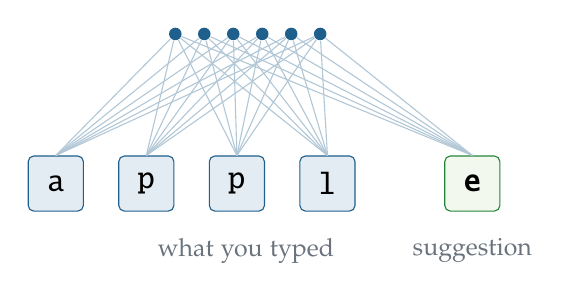
\begin{tikzpicture}[x=1.15cm,y=1cm,
  sym/.style={draw=accent, fill=titlebg, rounded corners=2pt, minimum width=0.7cm,
    minimum height=0.7cm, font=\ttfamily\large},
  dot/.style={circle, fill=accent, inner sep=1.6pt}]
  \foreach \c [count=\i] in {a,p,p,l} \node[sym] (s\i) at (\i,0) {\c};
  \node[sym, draw=st, fill=trybg, font=\ttfamily\bfseries\large] (q) at (5.6,0) {e};
  \foreach \j in {1,...,6} \node[dot] (h\j) at (2.0+0.32*\j,1.9) {};
  \foreach \i in {1,...,4} \foreach \j in {1,...,6} \draw[accent!35] (s\i.north) -- (h\j);
  \foreach \j in {1,...,6} \draw[accent!35] (h\j) -- (q.north);
  \node[font=\small, text=cm] at (3.1,-0.85) {what you typed};
  \node[font=\small, text=cm] at (5.6,-0.85) {suggestion};
\end{tikzpicture}

\vfill
{\large A step-by-step tutorial\par}
\vspace{0.3cm}
{\normalsize Every line of code, every equation, nothing hidden\par}
\vspace{1.5cm}
\end{titlepage}

\frontmatter
\tableofcontents
\mainmatter

% ===========================================================================
\chapter{What we are going to build}

Open a terminal, type the beginning of a word, and a program suggests how
to continue it, one letter at a time:

\begin{textout}
start of word> app
  app[r]   (23%)      others: e 19%, l 17%, o 15%, i 9%
  > l
  appl[e]   (45%)      others: i 19%, a 13%, y 11%, o 8%
  >
  apple[a]   (21%)      others: s 18%, r 11%, end 7%, n 7%
  > n
  apple[s]   (18%)      others: a 21%, r 11%, end 7%, n 7%
  >
  apples   -> looks complete (42%)      others: s 19%, t 15%, e 4%, h 4%
  >
  ==> apples
\end{textout}

After \code{app}, the program thinks \code{r} is the most likely next letter
(23\%), with \code{e} and \code{l} close behind. We typed \code{l}
ourselves to steer it. After \code{appl} it is fairly sure about \code{e}
(45\%), and we pressed Enter to accept. Then we asked for its second choice
with \code{n}, and accepted \code{s}. Finally the model judged
\code{apples} complete, and we agreed.

The thing making the suggestions is a \emph{neural network}: a few thousand
numbers, arranged in a particular way, that started out random and were
nudged, millions of times, until they got good at one job. The job is to
look at the last four letters of a word and give a probability for each
possible next letter.

This is, in miniature, exactly what a large language model does. A chatbot
looks at the text so far and gives a probability for each possible next
piece of text. The pieces are bigger (whole words or parts of words, not
letters), the network is far bigger (billions of numbers, not
thousands), and it looks much further back than four letters. But the
recipe is the same, and every ingredient of the recipe is in this small
project:
\begin{itemize}[nosep]
  \item turning symbols into vectors of numbers (\emph{embeddings});
  \item layers of artificial neurons;
  \item turning scores into probabilities (\emph{softmax});
  \item measuring how wrong a prediction is (\emph{cross-entropy loss});
  \item working out how to change every number to be a little less wrong
        (\emph{backpropagation});
  \item changing them, over and over (\emph{gradient descent}).
\end{itemize}

\section{How this tutorial works}

We will build the whole project together, from an empty folder, in small
steps. Each step adds a few lines of code to one of the project's files,
and explains what the code does and why. When there is math behind the
code, we work through the math first, in simple steps, and then turn it
into code.

The code comes in boxes like this one. The title of the box says which
file the code belongs to, and where in the file it goes:

\begin{tcolorbox}[codebox, title={\textbf{New file}\enspace\texttt{example.nex}}]
\small Start a new file with this content.
\end{tcolorbox}
\begin{tcolorbox}[codebox, title={\texttt{example.nex}\enspace\textendash\enspace add at the end}]
\small Add this code at the end of the file.
\end{tcolorbox}
\begin{tcolorbox}[codebox, title={\texttt{example.nex}\enspace\textendash\enspace add before the line ...}]
\small Add this code at a particular place in the file, which the title tells you.
\end{tcolorbox}
\begin{tcolorbox}[codebox, title={\texttt{example.nex}\enspace\textendash\enspace continued}]
\small Add this code right after the code from the previous box.
\end{tcolorbox}

Green boxes are \emph{try-it} scripts: small throwaway programs that use
what we just built, so you can see it working. Their output follows in a
dark box:

\begin{tcolorbox}[trybox, title={\textbf{Try it}\enspace\texttt{try\_example.nex}}]
\small A small program to run now. It is not part of the project.
\end{tcolorbox}
\begin{tcolorbox}[outbox]
{\ttfamily\footnotesize\color{outfg}\$ nex try\_example.nex\\what it prints}
\end{tcolorbox}

Every program and every output in this tutorial was produced by running
the code exactly as printed here, so if your output differs, compare your
code with the boxes. (Training on a different word list gives different
numbers, of course.)

\section{What you need}

\begin{itemize}[nosep]
  \item \textbf{Nex}, installed so that the \code{nex} command works in a
        terminal. You should know the basics of the language: \code{let},
        functions and \code{result}, classes, loops, and contracts
        (\code{require}, \code{ensure}, \code{invariant}). We explain the
        less common features as we meet them.
  \item \textbf{A word list}: a text file with one word per line. Linux and
        macOS have one at \path{/usr/share/dict/words}. Any other list
        works too.
  \item \textbf{Math}: school algebra. We will use vectors, matrices, the
        exponential and logarithm, and derivatives, and we explain each one
        when it first comes up. You don't need to have seen any of it in a
        long time.
\end{itemize}

No machine-learning library is used. Every multiplication, every
derivative and even the random number generator is written out in Nex,
in about 1,400 lines including comments and checks.

\section{The plan}

Here is the whole network, which the following chapters build one piece at
a time:

\begin{center}
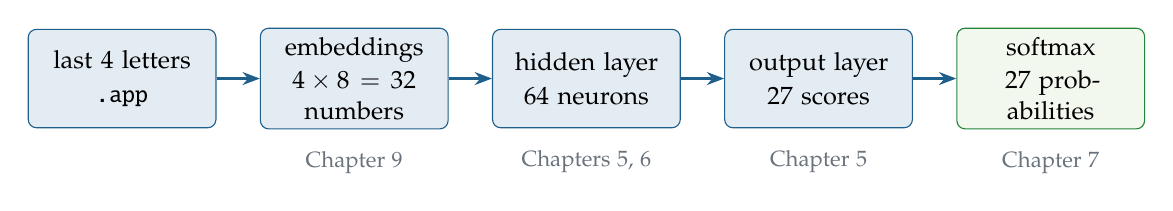
\begin{tikzpicture}[
  box/.style={draw=accent, fill=titlebg, rounded corners=3pt, align=center,
    minimum height=1.25cm, text width=2.15cm, font=\small},
  lab/.style={font=\footnotesize, text=cm, align=center},
  arr/.style={-{Stealth[length=2.2mm]}, thick, accent}]
  \node[box] (in) {last 4 letters\\[1pt]\texttt{.app}};
  \node[box, right=0.55cm of in] (emb) {embeddings\\[1pt]$4\times 8 = 32$\\numbers};
  \node[box, right=0.55cm of emb] (hid) {hidden layer\\[1pt]64 neurons};
  \node[box, right=0.55cm of hid] (out) {output layer\\[1pt]27 scores};
  \node[box, right=0.55cm of out, draw=st, fill=trybg] (sm) {softmax\\[1pt]27 probabilities};
  \draw[arr] (in) -- (emb);
  \draw[arr] (emb) -- (hid);
  \draw[arr] (hid) -- (out);
  \draw[arr] (out) -- (sm);
  \node[lab, below=0.15cm of emb] {Chapter 9};
  \node[lab, below=0.15cm of hid] {Chapters 5, 6};
  \node[lab, below=0.15cm of out] {Chapter 5};
  \node[lab, below=0.15cm of sm] {Chapter 7};
\end{tikzpicture}
\end{center}

\begin{enumerate}[nosep]
  \item[2--3.] Set up the project, and decide how to represent letters.
  \item[4--7.] The math toolkit: vectors, matrices, a squashing function,
        and softmax.
  \item[8--10.] Random numbers, the model itself, and running it forward.
  \item[11--15.] Training: the data, the loss, gradient descent,
        backpropagation, and checking that the gradients are right.
  \item[16--18.] Saving models, the training program, and the program you
        play with.
\end{enumerate}

By the end you will have these files, each of which you will have written
yourself:

\begin{center}
\small
\begin{tabular}{@{}ll@{}}
\toprule
File & What it holds \\
\midrule
\code{helpers.nex} & Printing numbers neatly, and finding files \\
\code{vocabulary.nex} & The 27 symbols the model knows \\
\code{vector_math.nex} & Dot products, layers, tanh, softmax \\
\code{rng.nex} & A random number generator \\
\code{next_letter_model.nex} & The neural network: forward pass, backpropagation, update \\
\code{training_data.nex} & Training examples, the loss, and evaluation \\
\code{checks.nex} & Automatic checks of everything, including the gradients \\
\code{train.nex} & The training program \\
\code{play.nex} & The word-completion program \\
\bottomrule
\end{tabular}
\end{center}

% ===========================================================================
\chapter{Setting up}

Make a folder for the project and go into it. Every file in this tutorial
goes in this one folder.

\begin{shell}
mkdir nextletter
cd nextletter
\end{shell}

\section{A first file: printing numbers}

We will print a lot of numbers along the way: probabilities, losses,
weights. Nex prints a \code{Real} with all its digits, like
\code{0.6652409557748218}, which is hard to read in a table. So the very
first file holds a few helpers for printing numbers neatly.

A Nex program uses another file with \code{intern}. \code{intern Helpers}
finds \code{helpers.nex} in the same folder and loads everything in it. The file does not need a class called \code{Helpers}:
ours holds only plain functions.

For a number with a fixed number of decimal places, Nex has the built-in
\code{format}, which gives text: \code{2.5.format(3)} is \code{"2.500"},
and \code{0.6652409557748218.format(3)} is \code{"0.665"}. It rounds to the
nearest, and a number exactly halfway rounds away from zero. (There is
also \code{to_fixed}, which rounds but gives back a \code{Real}, so
\code{2.5.to_fixed(3)} still prints as \code{2.5}.)

A small helper writes a probability as a percentage.

\begin{newfile}{helpers.nex}
-- helpers.nex: printing numbers neatly, and finding the user's files.

-- A probability as a whole percentage: percent(0.257) is "26%".
function percent(p: Real): String do
  result := (p * 100.0).round.to_string + "%"
end
\end{newfile}

To line up columns we will pad text to a fixed width with the built-in
\code{pad_start} (spaces on the left) and \code{pad_end} (spaces on the
right): \code{"42".pad_start(" ", 6)} puts four spaces in front of
\code{42}, making it 6 characters wide. Text that is already long enough
is left as it is.

And one that prints a whole list of numbers. It collects the numbers as
text in an array, and the built-in \code{join} glues them together with
\code{", "} between each pair:

\begin{append}{helpers.nex}
-- A list of numbers as text, each with `places` decimals:
-- vector_text([0.5, 0.25], 2) is "[0.50, 0.25]".
function vector_text(v: Array[Real], places: Integer): String do
  let parts: Array[String] := []
  across v as x do
    parts.add(x.format(places))
  end
  result := "[" + ", ".join(parts) + "]"
end
\end{append}

\section{Running a try-it script}

Let's check that it works. Make this file and run it:

\begin{tryit}{try_helpers.nex}
intern Helpers

console.print_line(2.5.format(3))
console.print_line((-3.14159).format(2))
console.print_line(percent(0.257))
console.print_line("[" + "42".pad_start(" ", 6) + "]")
console.print_line(vector_text([0.5, 0.25, 1.0 / 3.0], 3))
\end{tryit}
\tryoutput{try_helpers}

We print with \code{console.print_line}, because Nex's \code{print} shows
strings with their quotes (\code{"2.500"}), which is handy for debugging
but not for neat output. Every Nex program has \code{console}, a
\code{Console} that writes text as it is, without our having to create it.

Try-it scripts are not part of the project. Keep them around to experiment
with, or delete them when you are done.

% ===========================================================================
\chapter{Symbols}

A neural network only works with numbers. Before anything else, we decide
how letters become numbers.

Our model will predict one of 27 \emph{symbols}: the 26 letters
\code{a}\,\dots\,\code{z}, and one extra symbol, a full stop \code{.},
which does two jobs.

\begin{itemize}
  \item \textbf{It marks the end of a word.} To know when a word is
    finished, the model must be able to predict ``the word ends here''.
    After \code{apple}, the right answer is not a letter but \code{.}.
  \item \textbf{It pads the start of a word.} The model always looks at
    the last four symbols. At the start of a word there aren't four yet,
    so we fill the gap with full stops: before the first letter of
    \code{apple}, the model sees \code{....}, and the right answer is
    \code{a}. After \code{ap} it sees \code{..ap}.
\end{itemize}

Each symbol gets a number, its \emph{id}: \code{.} is 0, \code{a} is 1,
and so on up to \code{z}, which is 26. A Nex class can hold constants,
written \code{NAME = value}, which we read through the class name:
\code{Vocabulary.SIZE}.

\begin{newfile}{vocabulary.nex}
-- vocabulary.nex: the 27 symbols the model reads and predicts.
--
-- "." does two jobs:
--   * padding at the start, so even the first letter has a full context
--     ("...." -> "a" means "a word can start with a");
--   * the end-of-word marker, so the model can learn when to stop
--     ("appl" -> "e", then "pple" -> "." means "apple is complete").

class Vocabulary
feature
  END = "."
  SYMBOLS = ".abcdefghijklmnopqrstuvwxyz"
  SIZE = 27
end
\end{newfile}

The id of a symbol is simply its position in \code{SYMBOLS}, and the
symbol with a given id is the one-character piece of \code{SYMBOLS} at
that position:

\begin{append}{vocabulary.nex}
-- The id of a symbol: "." is 0, "a" is 1, ..., "z" is 26.
function symbol_id(ch: String): Integer
require
  one_symbol: ch.length = 1 and Vocabulary.SYMBOLS.contains(ch)
do
  result := Vocabulary.SYMBOLS.index_of(ch)
ensure
  in_range: result >= 0 and result < Vocabulary.SIZE
end

-- The symbol with a given id.
function symbol_at(id: Integer): String
require
  in_range: id >= 0 and id < Vocabulary.SIZE
do
  result := Vocabulary.SYMBOLS.substring(id, id + 1)
ensure
  one_symbol: result.length = 1
end
\end{append}

The contracts say exactly what these functions accept and promise.
\code{symbol_id} only accepts a single character that is one of our
symbols, and promises an id from 0 to 26. If some other part of the program
ever passes it a capital letter, the program stops right there, with a
message that names the broken promise, instead of carrying on with a
nonsense id and failing somewhere far away.

The word list we will train on contains words such as \code{Paris} and
\code{it's}, which use characters outside our 27 symbols. We'll skip those,
so we need a test for ``plain lowercase word''. A \emph{regular
expression} describes this exactly: \code{[a-z]+} means ``one or more
characters, each in the range \code{a} to \code{z}''. Nex's library has
regular expressions in \code{text/Regex}, so we intern that at the top of
the file:

\begin{addbefore}{vocabulary.nex}{at the top}{class Vocabulary}
intern text/Regex
\end{addbefore}

and use it:

\begin{append}{vocabulary.nex}
-- True when s is one or more of a..z, and nothing else.
function is_lowercase_word(s: String): Boolean do
  result := create Regex.compile("[a-z]+").matches(s)
end
\end{append}

\code{matches} is true only when the \emph{whole} string fits the pattern,
so \code{"it's"} fails because of the apostrophe, and the empty string
fails because \code{+} asks for at least one character.

\begin{tryit}{try_vocabulary.nex}
intern Vocabulary

console.print_line("symbols: " + Vocabulary.SYMBOLS)
console.print_line("id of a: " + symbol_id("a").to_string)
console.print_line("id of p: " + symbol_id("p").to_string)
console.print_line("symbol 16: " + symbol_at(16))
console.print_line("apple: " + is_lowercase_word("apple").to_string)
console.print_line("Paris: " + is_lowercase_word("Paris").to_string)
do
  console.print_line(symbol_id("A").to_string)
rescue
  console.print_line("symbol_id(\"A\") refused: " + exception.to_string)
end
\end{tryit}
\tryoutput{try_vocabulary}

The last lines show a contract at work: \code{symbol_id("A")} breaks the
precondition \code{one_symbol}, and the \code{rescue} block catches the
failure so that we can print it.

% ===========================================================================
\chapter{Vectors}

A neural network is mostly multiplication and addition, organized with
vectors and matrices. This chapter and the next build the small amount of
linear algebra we need.

\section{The math}

A \emph{vector} is a list of numbers. We write vectors in bold: a vector
$\vect{u}$ with $n$ numbers, or \emph{components}, is
\[
  \vect{u} = (u_0, u_1, \dots, u_{n-1}).
\]
We count from 0, as Nex arrays do. ``$\vect{u}$ is in $\R^n$'' is the
short way to say ``$\vect{u}$ is a list of $n$ real numbers''.

The single most important operation is the \emph{dot product} of two
vectors of the same length: multiply them component by component, and add
up the results.

\begin{mathbox}[Dot product]
\[
  \vect{u}\cdot\vect{v} \;=\; u_0 v_0 + u_1 v_1 + \dots + u_{n-1}v_{n-1}
  \;=\; \sum_{i=0}^{n-1} u_i v_i
\]
For example, $(1, 2, 3)\cdot(4, 5, 6) = 1\cdot 4 + 2\cdot 5 + 3\cdot 6 = 32$.
\end{mathbox}

The $\sum$ sign (capital sigma) means ``add up'': $\sum_{i=0}^{n-1} u_i v_i$
reads ``the sum of $u_i v_i$ for $i$ from 0 to $n-1$''.

Here is a way to think about the dot product that we will use all the
time. Suppose $\vect{v}$ holds some \emph{inputs}, and $\vect{u}$ holds a
\emph{weight} for each input. Then $\vect{u}\cdot\vect{v}$ is a
\emph{weighted sum} of the inputs: an input with a large positive weight
pushes the total up a lot, an input with a negative weight pulls it down,
and an input with weight zero is ignored. A shopping receipt is a dot
product: quantities times prices, added up.

\section{The code}

In Nex, a vector is an \code{Array[Real]}. Start the math file with a class
\code{Vector_Math} that holds one constant, which we will need in
Chapter~7.

\begin{newfile}{vector_math.nex}
-- vector_math.nex: the few pieces of linear algebra the network needs.
--
-- A vector is an Array[Real]. A matrix is an Array of rows, where each row
-- is a vector. No library does the math for us: every multiply and add is
-- written out below.

class Vector_Math
feature
  -- How far a sum of probabilities may drift from 1.0 through rounding.
  TOLERANCE = 1.0e-9
end
\end{newfile}

Two simple functions first: a vector of zeros, and the sum of a vector's
components.

\begin{append}{vector_math.nex}
-- A vector of n zeros.
function zeros(n: Integer): Array[Real]
require
  non_negative: n >= 0
do
  result := create Array.filled(n, 0.0)
ensure
  right_length: result.length = n
end

-- The sum of the elements.
function sum(v: Array[Real]): Real do
  across v as x do
    result := result + x
  end
end
\end{append}

\code{sum} relies on a Nex rule: \code{result} starts at the zero value of
its type, which is \code{0.0} for \code{Real}, so there is no need to set
it before the loop.

The dot product is the formula above, as a loop. Its precondition says
the two vectors must have the same length; otherwise the dot product isn't
defined.

\begin{append}{vector_math.nex}
-- The dot product: u[0]*v[0] + u[1]*v[1] + ...
function dot(u, v: Array[Real]): Real
require
  same_length: u.length = v.length
do
  from
    let i: Integer := 0
  until
    i = u.length
  do
    result := result + u.get(i) * v.get(i)
    i := i + 1
  end
end
\end{append}

\begin{tryit}{try_vectors.nex}
intern Vector_Math

let u: Array[Real] := [1.0, 2.0, 3.0]
let v: Array[Real] := [4.0, 5.0, 6.0]
console.print_line("zeros(3)  = " + zeros(3).to_string)
console.print_line("sum(u)    = " + sum(u).to_string)
console.print_line("dot(u, v) = " + dot(u, v).to_string)
do
  console.print_line(dot([1.0, 2.0], [1.0]).to_string)
rescue
  console.print_line("dot of different lengths: " + exception.to_string)
end
\end{tryit}
\tryoutput{try_vectors}

% ===========================================================================
\chapter{Matrices and layers}

\section{One neuron}

An artificial \emph{neuron} takes some inputs $x_0, \dots, x_{n-1}$, and
has a weight $w_j$ for each input and one extra number $b$, its
\emph{bias}. It computes the weighted sum of its inputs and adds the bias:
\[
  a = w_0 x_0 + w_1 x_1 + \dots + w_{n-1} x_{n-1} + b = \vect{w}\cdot\vect{x} + b.
\]

\begin{center}
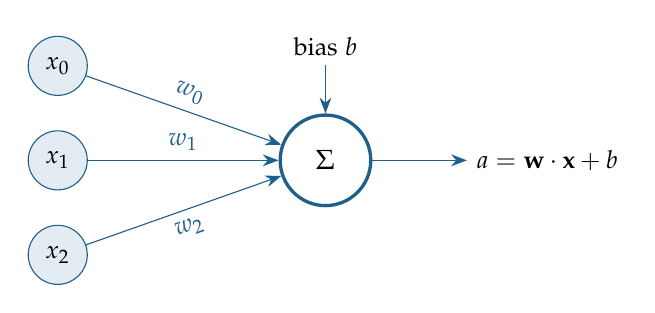
\begin{tikzpicture}[
  inp/.style={circle, draw=accent, fill=titlebg, minimum size=0.75cm, font=\small},
  neu/.style={circle, draw=accent, very thick, fill=white, minimum size=1.15cm},
  arr/.style={-{Stealth[length=2mm]}, accent}]
  \node[inp] (x0) at (0, 1.4) {$x_0$};
  \node[inp] (x1) at (0, 0.2) {$x_1$};
  \node[inp] (x2) at (0,-1.0) {$x_2$};
  \node[neu] (n) at (3.4, 0.2) {$\Sigma$};
  \draw[arr] (x0) -- node[above, font=\small, sloped] {$w_0$} (n);
  \draw[arr] (x1) -- node[above, font=\small] {$w_1$} (n);
  \draw[arr] (x2) -- node[below, font=\small, sloped] {$w_2$} (n);
  \node[font=\small] (b) at (3.4, 1.65) {bias $b$};
  \draw[arr] (b) -- (n);
  \node[font=\small, right=1.2cm of n] (a) {$a = \vect{w}\cdot\vect{x} + b$};
  \draw[arr] (n) -- (a);
\end{tikzpicture}
\end{center}

The weights decide which inputs the neuron cares about, and the bias
shifts its output up or down regardless of the inputs. Training a network
means finding good weights and biases.

\section{A layer of neurons is a matrix}

A \emph{layer} is several neurons that all read the same inputs, each with
its own weights and bias. If we write each neuron's weights as one row, we
get a table of numbers with one row per neuron and one column per input.
Such a table is a \emph{matrix}. A matrix with $m$ rows and $n$ columns is
an ``$m\times n$ matrix''. The number in row $i$, column $j$ of a matrix
$W$ is written $W_{ij}$.

Running the whole layer means taking the dot product of every row with the
input, and adding each row's bias. That is the \emph{matrix--vector
product} $W\vect{x}$, plus a bias vector $\vect{b}$:

\begin{mathbox}[A layer: $\vect{a} = W\vect{x} + \vect{b}$]
For an $m\times n$ matrix $W$, an input $\vect{x}\in\R^n$ and biases
$\vect{b}\in\R^m$, the output $\vect{a}\in\R^m$ has one component per row:
\[
  a_i = \sum_{j=0}^{n-1} W_{ij}\,x_j + b_i
      = (\text{row } i \text{ of } W)\cdot\vect{x} + b_i .
\]
For example,
\[
  \begin{pmatrix} 1 & 0 \\ 1 & 1 \end{pmatrix}
  \begin{pmatrix} 2 \\ 3 \end{pmatrix}
  + \begin{pmatrix} 0.5 \\ -1 \end{pmatrix}
  = \begin{pmatrix} 1\cdot 2 + 0\cdot 3 + 0.5 \\ 1\cdot 2 + 1\cdot 3 - 1 \end{pmatrix}
  = \begin{pmatrix} 2.5 \\ 4 \end{pmatrix}.
\]
\end{mathbox}

A function of the form $W\vect{x}+\vect{b}$ is called \emph{affine}. Our
network will have two layers like this: one with 64 neurons and 32 inputs
(a $64\times 32$ matrix), and one with 27 neurons, one per symbol, and 64
inputs (a $27\times 64$ matrix).

\section{The code}

In Nex, a matrix is an array of rows: \code{Array[Array[Real]]}. First, a
matrix of zeros. It builds each row with its own call to \code{zeros}, so
that every row is a separate array. (If all rows were the same array,
changing one would change them all.)

\begin{append}{vector_math.nex}
-- A rows x cols matrix of zeros. Each row is its own array, so changing
-- one row never changes another.
function zero_matrix(rows, cols: Integer): Array[Array[Real]]
require
  non_negative: rows >= 0 and cols >= 0
do
  repeat rows do
    result.add(zeros(cols))
  end
ensure
  right_rows: result.length = rows
end
\end{append}

Then the layer itself. It is a dot product per row, exactly as in the box
above:

\begin{append}{vector_math.nex}
-- W·x + b: one dot product per row of W, plus that row's bias.
-- Each row is one neuron; all the rows together are a layer.
function affine(w: Array[Array[Real]], x, b: Array[Real]): Array[Real]
require
  one_bias_per_row: w.length = b.length
do
  from
    let i: Integer := 0
  until
    i = w.length
  do
    result.add(dot(w.get(i), x) + b.get(i))
    i := i + 1
  end
ensure
  one_output_per_row: result.length = w.length
end
\end{append}

One more operation, which looks modest but will do most of the work in
training: add a multiple of one vector to another, in place,
$\vect{t} \leftarrow \vect{t} + s\,\vect{v}$. (The arrow means ``becomes''.)

\begin{append}{vector_math.nex}
-- target := target + s * v, changing target in place.
-- Backpropagation and gradient descent are built almost entirely from this.
function add_scaled(target: Array[Real], s: Real, v: Array[Real])
require
  same_length: target.length = v.length
do
  from
    let i: Integer := 0
  until
    i = target.length
  do
    target.set(i, target.get(i) + s * v.get(i))
    i := i + 1
  end
end
\end{append}

\begin{tryit}{try_layer.nex}
intern Vector_Math
intern Helpers

-- The example from the box: two neurons with two inputs each.
let w: Array[Array[Real]] := [[1.0, 0.0], [1.0, 1.0]]
let x: Array[Real] := [2.0, 3.0]
let b: Array[Real] := [0.5, -1.0]
console.print_line("W x + b = " + vector_text(affine(w, x, b), 1))

let t: Array[Real] := [1.0, 1.0]
add_scaled(t, 0.5, [2.0, 4.0])
console.print_line("[1, 1] + 0.5 * [2, 4] = " + vector_text(t, 1))
console.print_line("a 2 x 3 zero matrix: " + zero_matrix(2, 3).to_string)
\end{tryit}
\tryoutput{try_layer}

% ===========================================================================
\chapter{Bending the line: tanh}

\section{Why layers alone are not enough}

If we put two affine layers one after the other, something disappointing
happens. Feed $\vect{x}$ to the first layer, and its output to the second:
\[
  W_2(W_1\vect{x} + \vect{b}_1) + \vect{b}_2
  \;=\; (W_2 W_1)\,\vect{x} + (W_2\vect{b}_1 + \vect{b}_2).
\]
The result is again of the form (some matrix)$\cdot\vect{x}$ + (some
vector): two affine layers are no more powerful than one. However many we
stack, we only ever get an affine function, and affine functions can only
describe straight-line (``linear'') relationships. Predicting spelling
needs much more than that.

The fix is to pass each neuron's output through a \emph{nonlinear}
function before the next layer. This function is called the
\emph{activation function}, and it is what lets a network describe curved,
complicated relationships. We use the \emph{hyperbolic tangent}, $\tanh$.

\section{The math of tanh}

\begin{mathbox}[The hyperbolic tangent]
\[
  \tanh(v) = \frac{e^{v} - e^{-v}}{e^{v} + e^{-v}}
\]
\end{mathbox}

Here $e \approx 2.718$ is Euler's number, and $e^v$ is the
\emph{exponential} function: it is always positive, it is 1 at $v=0$, it
grows very fast for positive $v$ ($e^{10}\approx 22026$), and it shrinks
toward 0 for negative $v$.

\begin{center}
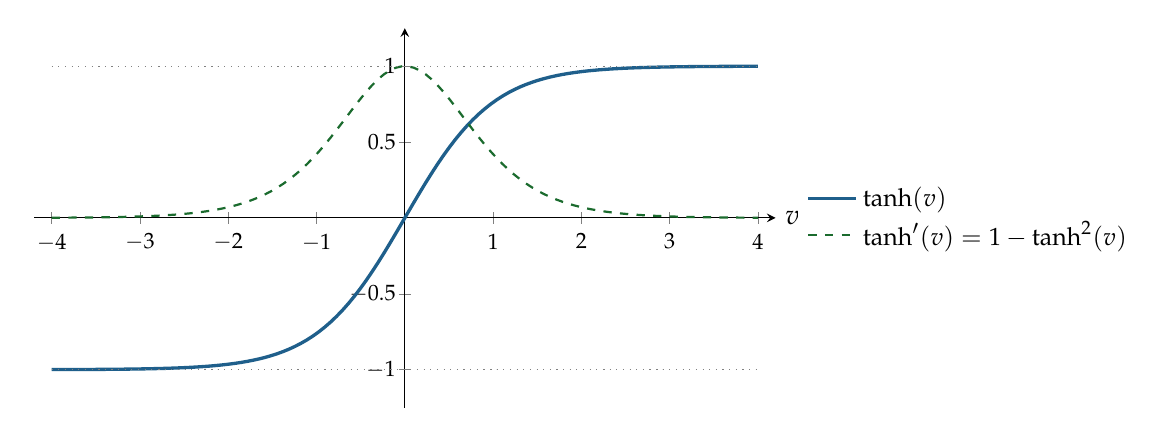
\begin{tikzpicture}
\begin{axis}[width=11cm, height=6.4cm, axis lines=middle, xmin=-4.2, xmax=4.2,
  ymin=-1.25, ymax=1.25, xtick={-4,-3,-2,-1,1,2,3,4}, ytick={-1,-0.5,0.5,1},
  xlabel={$v$}, every axis x label/.style={at={(ticklabel* cs:1.0)}, anchor=west},
  yticklabel style={fill=white, inner sep=1pt},
  legend style={draw=none, fill=white, font=\small, at={(1.03,0.5)}, anchor=west},
  legend cell align=left,
  tick label style={font=\footnotesize}, samples=120, domain=-4:4]
  \addplot[very thick, accent] {tanh(x)};
  \addlegendentry{$\tanh(v)$}
  \addplot[thick, dashed, st!80!black] {1 - tanh(x)^2};
  \addlegendentry{$\tanh'(v) = 1-\tanh^2(v)$}
  \addplot[thin, gray, dotted, domain=-4:4, forget plot] {1};
  \addplot[thin, gray, dotted, domain=-4:4, forget plot] {-1};
\end{axis}
\end{tikzpicture}
\end{center}

The solid curve is $\tanh$. It is close to a straight line near zero
($\tanh(v)\approx v$ for small $v$), and it flattens out toward $+1$ for
large positive $v$ and toward $-1$ for large negative $v$. So it
\emph{squashes} any number into the range $(-1, 1)$. A neuron followed by
$\tanh$ behaves like a soft switch: strongly negative input means
``off'' ($-1$), strongly positive input means ``on'' ($+1$), and in between
it responds smoothly.

\subsection{A form that is safe to compute}

The formula above has a practical problem. For $v = 1000$, $e^{1000}$ is
far too big for a computer's floating-point numbers: it becomes
\code{Infinity}, and $\infty/\infty$ is not a number at all. Let's rewrite
the formula. Multiply the top and the bottom by $e^{v}$:
\[
  \tanh(v) = \frac{e^{2v} - 1}{e^{2v} + 1}
           = \frac{(e^{2v} + 1) - 2}{e^{2v} + 1}
           = 1 - \frac{2}{e^{2v} + 1}.
\]
The last form is safe. For large $v$, $e^{2v}$ becomes \code{Infinity},
$2/\infty = 0$, and the answer is exactly $1$, which is correct. For very
negative $v$, $e^{2v}$ becomes 0, and the answer is $1 - 2 = -1$, also
correct.

\subsection{The derivative}

Training will need to know how fast $\tanh$ changes, which is its
\emph{derivative}. (Chapter~12 reviews derivatives; for now, the
derivative of a function at a point is the slope of its graph there.) The
derivative of $\tanh$ has a remarkably simple form:

\begin{mathbox}[Derivative of tanh]
\[
  \tanh'(v) = 1 - \tanh^2(v)
\]
\end{mathbox}

To see why, write $\tanh(v) = s/c$ with $s = e^{v} - e^{-v}$ and
$c = e^{v} + e^{-v}$. Since the derivative of $e^{v}$ is $e^{v}$ and the
derivative of $e^{-v}$ is $-e^{-v}$, we get $s' = c$ and $c' = s$. The
quotient rule $(s/c)' = (s'c - sc')/c^2$ gives
\[
  \tanh'(v) = \frac{c\cdot c - s\cdot s}{c^2} = 1 - \frac{s^2}{c^2} = 1 - \tanh^2(v).
\]

The dashed curve in the plot is this derivative. It is 1 at $v = 0$, where
$\tanh$ is steepest, and nearly 0 far from zero, where $\tanh$ is flat.
The nice thing about this form is that once we have computed
$h = \tanh(v)$, the derivative costs one multiplication: $1 - h^2$.

\section{The code}

\code{Real} in Nex has \code{exp}, but no \code{tanh}, so we write it
ourselves, using the safe form:

\begin{append}{vector_math.nex}
-- The hyperbolic tangent, squashing any real number into (-1, 1).
-- Real has no tanh method, so we build it from exp:
--     tanh(v) = (e^2v - 1) / (e^2v + 1) = 1 - 2 / (e^2v + 1)
-- The second form is safe for large v: e^2v overflows to Infinity,
-- 2 / Infinity is 0, and the answer is exactly 1.
function tanh(v: Real): Real
do
  result := 1.0 - 2.0 / ((2.0 * v).exp + 1.0)
ensure
  bounded: result >= -1.0 and result <= 1.0
end
\end{append}

\begin{tryit}{try_tanh.nex}
intern Vector_Math
intern Helpers

console.print_line("     v    tanh(v)   1 - tanh(v)^2")
across [-3.0, -1.0, -0.1, 0.0, 0.1, 1.0, 3.0] as v do
  let h: Real := tanh(v)
  console.print_line(v.format(1).pad_start(" ", 6) + h.format(4).pad_start(" ", 11)
    + (1.0 - h * h).format(4).pad_start(" ", 16))
end
console.print_line("tanh(1000)  = " + tanh(1000.0).to_string)
console.print_line("tanh(-1000) = " + tanh(-1000.0).to_string)
\end{tryit}
\tryoutput{try_tanh}

Near zero, $\tanh(0.1) \approx 0.0997$, almost exactly $0.1$: there,
$\tanh$ is nearly a straight line. At $\pm 3$, the derivative has dropped
to about $0.01$: the curve is almost flat.

% ===========================================================================
\chapter{From scores to probabilities: softmax}

The last layer of our network has 27 neurons, one per symbol. Their
outputs are 27 arbitrary numbers, called \emph{scores} or \emph{logits}:
a high score means ``this symbol is likely''. But what we want is
probabilities: 27 numbers between 0 and 1 that add up to 1.

\section{The math}

The \emph{softmax} function does this conversion. It makes every score
positive by taking its exponential, and then divides by the total, so the
results add up to 1:

\begin{mathbox}[Softmax]
For scores $\vect{z} = (z_0, \dots, z_{K-1})$,
\[
  p_i = \operatorname{softmax}(\vect{z})_i = \frac{e^{z_i}}{\sum_{j=0}^{K-1} e^{z_j}} .
\]
Every $p_i$ is positive, and $\sum_i p_i = 1$.
\end{mathbox}

For example, take scores $(2.0, 1.0, 0.1)$. The exponentials are
$e^{2.0} \approx 7.389$, $e^{1.0} \approx 2.718$ and
$e^{0.1} \approx 1.105$, which add up to $11.212$. Dividing each by the
total gives the probabilities $(0.659, 0.242, 0.099)$.

\begin{center}
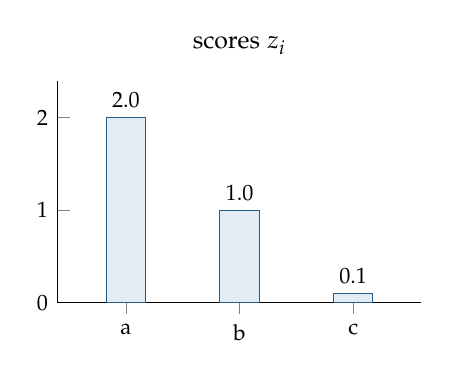
\begin{tikzpicture}
\begin{axis}[ybar, width=6.2cm, height=4.4cm, bar width=0.5cm, ymin=0, ymax=2.4,
  symbolic x coords={a,b,c}, xtick=data, title={\small scores $z_i$},
  nodes near coords, point meta=explicit symbolic, every node near coord/.append style={font=\footnotesize},
  tick label style={font=\footnotesize}, axis lines*=left, enlarge x limits=0.3]
  \addplot[fill=titlebg, draw=accent] coordinates {(a,2.0) [2.0] (b,1.0) [1.0] (c,0.1) [0.1]};
\end{axis}
\end{tikzpicture}
\hspace{0.4cm}\raisebox{1.6cm}{$\xrightarrow{\ \text{softmax}\ }$}\hspace{0.4cm}
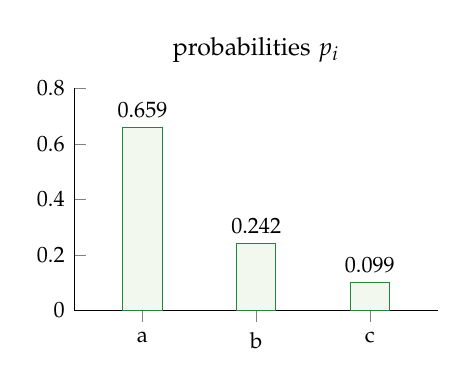
\begin{tikzpicture}
\begin{axis}[ybar, width=6.2cm, height=4.4cm, bar width=0.5cm, ymin=0, ymax=0.8,
  symbolic x coords={a,b,c}, xtick=data, title={\small probabilities $p_i$},
  nodes near coords, point meta=explicit symbolic, every node near coord/.append style={font=\footnotesize},
  tick label style={font=\footnotesize}, axis lines*=left, enlarge x limits=0.3]
  \addplot[fill=trybg, draw=st] coordinates {(a,0.659) [0.659] (b,0.242) [0.242] (c,0.099) [0.099]};
\end{axis}
\end{tikzpicture}
\end{center}

Notice that the exponential exaggerates differences: the scores 2.0 and
1.0 differ by 1, and their probabilities differ by a factor of
$e^1 \approx 2.7$. In general, adding 1 to a score multiplies that
symbol's (unnormalized) weight by $e$.

\subsection{Shifting the scores changes nothing}

If we add the same number $c$ to every score, the probabilities stay
exactly the same:
\[
  \frac{e^{z_i + c}}{\sum_j e^{z_j + c}}
  = \frac{e^{c}\, e^{z_i}}{e^{c}\sum_j e^{z_j}}
  = \frac{e^{z_i}}{\sum_j e^{z_j}} ,
\]
because $e^{c}$ appears on the top and on every term of the bottom, and
cancels. This matters for the same reason as with $\tanh$: $e^{z}$
overflows to infinity once $z$ is bigger than about 709. So before taking
exponentials, we subtract the largest score, $m = \max_j z_j$, from every
score. Then the largest exponent is $e^0 = 1$, nothing can overflow, and
the answer is unchanged.

\section{The code}

\begin{append}{vector_math.nex}
-- Turn raw scores ("logits") into probabilities that sum to 1.
-- Subtracting the largest score first changes nothing in the answer
-- (it cancels between top and bottom), but it keeps exp from
-- overflowing when a score is large.
function softmax(z: Array[Real]): Array[Real]
require
  not_empty: z.length > 0
do
  let m: Real := z.get(0)
  across z as v do
    m := m.max(v)
  end
  let exps: Array[Real] := []
  across z as v do
    exps.add((v - m).exp)
  end
  let total: Real := sum(exps)
  across exps as e do
    result.add(e / total)
  end
ensure
  same_length: result.length = z.length
  sums_to_one: (sum(result) - 1.0).abs < Vector_Math.TOLERANCE
end
\end{append}

The postcondition \code{sums_to_one} is where the \code{TOLERANCE}
constant comes in. Floating-point arithmetic rounds a little at every
step, so the sum may come out as \code{0.9999999999999999} instead of
exactly 1. The contract allows a tiny difference, and nothing more. Every
time the network runs, this contract checks that our probabilities really
are probabilities.

We will also want the position of the largest number in a vector: the
network's top choice.

\begin{append}{vector_math.nex}
-- The index of the largest element (the first one, if there is a tie).
function argmax(v: Array[Real]): Integer
require
  not_empty: v.length > 0
do
  from
    let i: Integer := 1
  until
    i = v.length
  do
    if v.get(i) > v.get(result) then
      result := i
    end
    i := i + 1
  end
ensure
  in_range: result >= 0 and result < v.length
end
\end{append}

\begin{tryit}{try_softmax.nex}
intern Vector_Math
intern Helpers

let p: Array[Real] := softmax([2.0, 1.0, 0.1])
console.print_line("softmax([2.0, 1.0, 0.1]) = " + vector_text(p, 3))
console.print_line("sum = " + sum(p).to_string)
let shifted: Array[Real] := softmax([1002.0, 1001.0, 1000.1])
console.print_line("scores shifted by 1000  = " + vector_text(shifted, 3))
console.print_line("equal scores            = " + vector_text(softmax([5.0, 5.0, 5.0, 5.0]), 3))
console.print_line("argmax = " + argmax(p).to_string)
\end{tryit}
\tryoutput{try_softmax}

Scores of 1000 and more would overflow without the shift; with it, we get
the same probabilities as before. And equal scores give equal
probabilities, as they should.

% ===========================================================================
\chapter{Randomness}

A new network starts with random weights. (If all weights started equal,
all the neurons in a layer would compute the same thing, receive the same
updates, and stay identical forever. Randomness breaks the tie.) Training
also picks examples at random. We want this randomness to be
\emph{repeatable}: two runs with the same \emph{seed} should produce
exactly the same ``random'' numbers, so that a result can be reproduced
and a bug can be chased. So we write our own small random number
generator.

\section{Uniform numbers: Park--Miller}

The idea of a \emph{pseudo-random} generator is to keep a hidden number,
the \emph{state}, and to update it with a fixed formula every time we want
a new number. The formula is chosen so that the sequence of states looks
random. One of the simplest good formulas is the Park--Miller ``minimal
standard'' generator:

\begin{mathbox}[Park--Miller generator]
\[
  \text{state} \leftarrow (\text{state} \times 48271) \bmod M,
  \qquad M = 2^{31} - 1 = 2147483647 .
\]
\end{mathbox}

``$a \bmod M$'' is the remainder after dividing $a$ by $M$, written
\texttt{a \% M} in Nex. Because $M$ is a prime number, and $48271$ is
carefully chosen, the state runs through every number from 1 to $M-1$, in
a scrambled order, before it repeats. It must never be 0, since 0 would
stay 0 forever.

There is one more thing to check. Nex's \code{Integer} has 64 bits, and
arithmetic that goes past $2^{63}$ is an error, not a silent wrap-around.
The state is always less than $M < 2^{31}$, and $48271 < 2^{16}$, so the
product is less than $2^{47}$. It always fits.

To get a real number between 0 and 1, divide the state by $M$. Since the
state is between 1 and $M-1$, the result is strictly between 0 and 1,
never exactly 0 or 1. (We will take its logarithm in a moment, and
$\ln 0$ is $-\infty$, so this matters.)

\begin{newfile}{rng.nex}
-- rng.nex: a small random number generator that can be seeded.
--
-- Neural networks start from random weights and learn from randomly
-- chosen examples. With a seed, the "random" numbers are the same on every
-- run, so a training run can be repeated exactly.
--
-- This is the Park-Miller "minimal standard" generator:
--     state := state * 48271 mod (2^31 - 1)
-- 2^31 - 1 is prime, and every state stays below it, so state * 48271 is
-- less than 2^47 and never overflows a 64-bit Integer.

class Rng
create
  make(seed: Integer) do
    -- Map any seed into the valid range 1 .. MODULUS - 1 (0 would stick).
    state := 1 + seed.abs % (MODULUS - 1)
  end
feature
  MODULUS = 2147483647
  MULTIPLIER = 48271

  state: Integer

  -- A real number spread evenly over the open interval (0, 1).
  uniform(): Real
  do
    state := (state * MULTIPLIER) % MODULUS
    result := state.to_real / MODULUS.to_real
  ensure
    open_interval: result > 0.0 and result < 1.0
  end

invariant
  state_in_range: state >= 1 and state < MODULUS
end
\end{newfile}

The class invariant \code{state_in_range} is checked after the object is
created and around every call to it, so a state of 0 could never sneak in.

\section{Whole numbers}

To pick a random example out of $n$, we need a whole number from $0$ to
$n-1$. Multiply a uniform number $u \in (0,1)$ by $n$ and round down:
$\lfloor u\,n \rfloor$. Since $0 < u\,n < n$, the result is one of
$0, 1, \dots, n-1$, each about equally likely.

\begin{addbefore}{rng.nex}{before the invariant}{invariant}
  -- A whole number in 0 .. n - 1, each equally likely.
  below(n: Integer): Integer
  require
    positive: n > 0
  do
    result := (uniform() * n.to_real).floor
  ensure
    in_range: result >= 0 and result < n
  end
\end{addbefore}

\section{Bell-curve numbers: Box--Muller}

Starting weights are usually drawn from the \emph{normal distribution},
the familiar bell curve: most values near 0, fewer and fewer further out.
A \emph{standard} normal number has mean (average) 0 and standard
deviation 1, which means that about 68\% of the values are between $-1$
and $1$, and about 95\% are between $-2$ and $2$.

The Box--Muller transform makes two standard normal numbers out of two
uniform numbers $u_1, u_2 \in (0, 1)$:

\begin{mathbox}[Box--Muller transform]
\[
  r = \sqrt{-2\ln u_1}, \qquad \theta = 2\pi u_2, \qquad
  z_1 = r\cos\theta, \qquad z_2 = r\sin\theta .
\]
\end{mathbox}

Why does this work? Picture a point $(z_1, z_2)$ whose two coordinates
are independent standard normal numbers: a cloud of points, densest at the
origin. The cloud is perfectly round, so the direction $\theta$ of a point
is equally likely to be any angle: that is $2\pi u_2$. Its distance $r$
from the origin is not uniform; a calculation in polar coordinates shows
that $r^2$ follows the \emph{exponential} distribution with mean 2, and
$-2\ln u_1$ is exactly how to make such a number from a uniform one. Then
$r\cos\theta$ and $r\sin\theta$ turn the polar coordinates back into
$z_1$ and $z_2$.

The transform gives two numbers at a time. We return the first and keep
the second, the \emph{spare}, for the next call:

\begin{addbefore}{rng.nex}{before the invariant}{invariant}
  -- Box-Muller (below) makes normal numbers in pairs; this holds the
  -- second one until it is asked for.
  has_spare: Boolean
  spare: Real

  -- A number from the standard normal ("bell curve") distribution, with
  -- mean 0 and standard deviation 1, by the Box-Muller transform: two
  -- uniform numbers u1, u2 give two independent normal numbers
  --     sqrt(-2 ln u1) * cos(2 pi u2)   and   sqrt(-2 ln u1) * sin(2 pi u2)
  gauss(): Real do
    if has_spare then
      has_spare := false
      result := spare
    else
      let radius: Real := (-2.0 * uniform().log).sqrt
      let angle: Real := 2.0 * Real.PI * uniform()
      spare := radius * angle.sin
      has_spare := true
      result := radius * angle.cos
    end
  end
\end{addbefore}

\section{Shuffling}

Finally, we need to shuffle a list: to split words fairly into a training
set and a test set. The \emph{Fisher--Yates} shuffle walks from the last
position to the first, and swaps the element at each position $i$ with a
randomly chosen element at a position $j$ from $0$ to $i$ (possibly $i$
itself). The last position gets each of the $n$ elements with equal
chance, the one before it gets each of the remaining $n-1$, and so on, so
each of the $n!$ possible orders is equally likely.

The function is \emph{generic}: \code{[T]} means it works on an array of
anything, words or training examples. (Nex allows generic functions but
not generic methods, so it is a function that takes the generator as an
argument.)

\begin{append}{rng.nex}
-- Shuffle an array in place (Fisher-Yates): walk from the end, swapping
-- each element with a randomly chosen one at or before it.
function shuffle[T](rng: Rng, items: Array[T]) do
  from
    let i: Integer := items.length - 1
  until
    i <= 0
  do
    let j: Integer := rng.below(i + 1)
    let tmp: T := items.get(i)
    items.set(i, items.get(j))
    items.set(j, tmp)
    i := i - 1
  end
end
\end{append}

\begin{tryit}{try_rng.nex}
intern Rng
intern Helpers

let rng: Rng := create Rng.make(42)
console.print_line("uniform: " + rng.uniform().format(4) + " " + rng.uniform().format(4))
console.print_line("below(10): " + rng.below(10).to_string + " " + rng.below(10).to_string)

-- Draw many normal numbers and measure their mean and spread.
let n: Integer := 100000
let total: Real := 0.0
let squares: Real := 0.0
let within_one: Integer := 0
repeat n do
  let z: Real := rng.gauss()
  total := total + z
  squares := squares + z * z
  if z.abs < 1.0 then
    within_one := within_one + 1
  end
end
let mean: Real := total / n.to_real
console.print_line("mean " + mean.format(3) + ", standard deviation "
  + (squares / n.to_real - mean * mean).sqrt.format(3)
  + ", within 1 of the mean: " + percent(within_one.to_real / n.to_real))

let words: Array[String] := ["one", "two", "three", "four", "five"]
shuffle(rng, words)
console.print_line("shuffled: " + words.to_string)
let again: Rng := create Rng.make(42)
console.print_line("same seed again: " + again.uniform().format(4))
\end{tryit}
\tryoutput{try_rng}

The normal numbers have mean close to 0, standard deviation close to 1,
and about 68\% of them fall within 1 of the mean, as the bell curve
predicts. And a new generator with the same seed starts the same sequence
again.

% ===========================================================================
\chapter{The model}

We now have all the tools to build the network itself. This chapter sets
up its parameters; the next one runs it.

\section{Embeddings: letters as vectors}

How do we feed a letter to a layer? A layer wants a vector of numbers. We
could feed the id itself, say 16 for \code{p}, but that would suggest that
\code{p} (16) is ``more'' than \code{a} (1), and close to \code{o} (15),
which is meaningless.

Instead, every symbol gets its own vector of 8 numbers, called its
\emph{embedding}. The 27 embeddings are the rows of a $27\times 8$ matrix
$C$. To feed a letter to the network, we look up its row: the letter with
id $s$ becomes row $s$ of $C$, written $C_s$.

The crucial point is that the embeddings are \emph{learned}. They start
out random, and training adjusts them like every other weight. Letters
that behave alike (say, the vowels) tend to end up with similar vectors,
because that helps the network make good predictions. Nobody tells it to
do this.

Looking up a row is a matrix operation in disguise. Write the symbol as a
\emph{one-hot} vector $\vect{e}_s$ with 27 components, all 0 except a 1 in
position $s$. Then
\[
  C^{\mathsf T}\vect{e}_s = C_s ,
\]
where $C^{\mathsf T}$, the \emph{transpose} of $C$, is $C$ with rows and
columns swapped: multiplying by a one-hot vector picks out one column of
$C^{\mathsf T}$, which is one row of $C$. So an embedding is just a layer
without bias, applied to a one-hot input. Looking the row up directly
gives the same answer without multiplying by 26 zeros.

The model looks at the last 4 symbols. Their 4 embeddings, joined end to
end, make the input vector $\vect{x}$ with $4 \times 8 = 32$ components:
\[
  \vect{x} = (C_{s_1}, C_{s_2}, C_{s_3}, C_{s_4}) \in \R^{32} .
\]

\section{The whole network}

\begin{mathbox}[The forward pass]
For context symbols $s_1, \dots, s_4$:
\begin{align*}
  \vect{x} &= (C_{s_1}, C_{s_2}, C_{s_3}, C_{s_4}) && \text{embeddings, } \R^{32}\\
  \vect{a} &= W_1\vect{x} + \vect{b}_1 && \text{hidden layer, } \R^{64}\\
  \vect{h} &= \tanh(\vect{a}) && \text{applied to each component}\\
  \vect{z} &= W_2\vect{h} + \vect{b}_2 && \text{output layer, } \R^{27}\\
  \vect{p} &= \operatorname{softmax}(\vect{z}) && \text{probabilities}
\end{align*}
\end{mathbox}

The numbers that training adjusts are the \emph{parameters}: $C$
($27\times 8$), $W_1$ ($64\times 32$), $\vect{b}_1$ (64), $W_2$
($27\times 64$) and $\vect{b}_2$ (27). In total:
\[
  27\cdot 8 + 64\cdot 32 + 64 + 27\cdot 64 + 27
  = 216 + 2048 + 64 + 1728 + 27 = 4083 .
\]
The sizes 4 (context), 8 (embedding) and 64 (hidden neurons) are not
learned; we choose them. Such choices are called \emph{hyperparameters}.

\section{Choosing the starting values}

The starting weights are random, but their \emph{size} matters. Consider
one hidden neuron before $\tanh$:
$a_i = \sum_{j} W_{1,ij}\, x_j$ (the biases start at 0). Suppose each
$x_j$ has mean 0 and variance 1 (the embeddings are standard normal) and
each weight is a normal number times a scale $\sigma$. For independent
quantities with mean 0, variances add, and the variance of a product of
two of them is the product of their variances. So
\[
  \operatorname{Var}(a_i) = \sum_{j=0}^{n-1} \operatorname{Var}(W_{1,ij})\operatorname{Var}(x_j)
  = n\,\sigma^2 ,
\]
where $n = 32$ is the number of inputs. (The variance is the square of the
standard deviation: a measure of spread.) If we used $\sigma = 1$, the
$a_i$ would have a standard deviation of $\sqrt{32}\approx 5.7$, so most
neurons would start deep in the flat parts of $\tanh$, where its
derivative is nearly 0 and, as we will see, learning is very slow. With
$\sigma = 1/\sqrt{n}$ the variance is exactly 1: the neurons start in the
lively middle part of $\tanh$.

For the output layer we want the opposite: very small scores, so that
softmax gives every symbol about the same probability, $1/27$. That is an
honest start: the untrained model knows nothing, so it should not have
strong opinions. We use $\sigma = 0.1/\sqrt{64}$, which gives scores with
a standard deviation of at most 0.1.

\section{The code}

The model file starts with the files it uses. It also interns two
libraries, \code{data/Json} and \code{io/Path}, which we will need in
Chapter~16 for saving the model to a file.

The constructor \code{make} takes the three hyperparameters and a seed,
and sets up all the parameters as described. The fields are listed after
it, and the invariant states their shapes, so a parameter matrix with the
wrong number of rows is caught immediately.

\begin{newfile}{next_letter_model.nex}
-- next_letter_model.nex: a tiny neural network that predicts the next
-- letter of a word.
--
-- It reads the last few letters of a partly typed word and gives a
-- probability for each of the 27 symbols (a..z, and "." for "the word is
-- finished").
--
--   last 4 letters --> embeddings --> hidden layer --> output layer --> softmax
--     (ids)           4 x 8 = 32       64 neurons      27 logits       27 probs
--                     lookup in C    tanh(W1·x + b1)   W2·h + b2

intern Vector_Math
intern Vocabulary
intern Rng
intern data/Json
intern io/Path

class Next_Letter_Model
create
  -- A fresh, untrained model with random weights.
  make(context, emb_dim, hidden, seed: Integer)
  require
    positive_sizes: context > 0 and emb_dim > 0 and hidden > 0
  do
    -- Hyperparameters: chosen by us, not learned.
    this.context := context
    this.emb_dim := emb_dim
    this.hidden := hidden

    -- Parameters: learned during training. They start out random.
    let rng: Rng := create Rng.make(seed)
    let n_in: Integer := context * emb_dim

    -- C: one embedding row per symbol.
    c := random_matrix(rng, Vocabulary.SIZE, emb_dim, 1.0)

    -- W1, b1: the hidden layer. Scaling by 1/sqrt(n_in) keeps W1·x
    -- small at the start, where tanh is not yet flat.
    w1 := random_matrix(rng, hidden, n_in, 1.0 / n_in.to_real.sqrt)
    b1 := zeros(hidden)

    -- W2, b2: the output layer. Tiny weights make every symbol start
    -- out about equally likely: an honest "I know nothing yet".
    w2 := random_matrix(rng, Vocabulary.SIZE, hidden, 0.1 / hidden.to_real.sqrt)
    b2 := zeros(Vocabulary.SIZE)
  end

feature
  context: Integer   -- how many previous letters the model sees
  emb_dim: Integer   -- length of each letter's embedding vector
  hidden: Integer    -- number of neurons in the hidden layer

  c: Array[Array[Real]]    -- embeddings,   Vocabulary.SIZE x emb_dim
  w1: Array[Array[Real]]   -- hidden layer, hidden x (context * emb_dim)
  b1: Array[Real]          --               hidden
  w2: Array[Array[Real]]   -- output layer, Vocabulary.SIZE x hidden
  b2: Array[Real]          --               Vocabulary.SIZE

invariant
  embedding_rows: c.length = Vocabulary.SIZE
  hidden_rows: w1.length = hidden and b1.length = hidden
  output_rows: w2.length = Vocabulary.SIZE and b2.length = Vocabulary.SIZE
end
\end{newfile}

In the constructor, a parameter has the same name as a field
(\code{context}). Inside the constructor, \code{context} means the
parameter, and \code{this.context} means the field.

\code{random_matrix} makes a matrix of normal numbers, each multiplied by
a scale:

\begin{append}{next_letter_model.nex}
-- A rows x cols matrix of normal random numbers, each times `scale`.
function random_matrix(rng: Rng, rows, cols: Integer, scale: Real): Array[Array[Real]]
do
  repeat rows do
    let row: Array[Real] := []
    repeat cols do
      row.add(rng.gauss() * scale)
    end
    result.add(row)
  end
ensure
  right_rows: result.length = rows
end
\end{append}

Two small methods complete the setup. The first turns the end of a typed
word into the 4 ids the network reads. We pad the word with \code{context}
full stops on the left, and then take its last \code{context} characters:
\code{"app"} becomes \code{"....app"}, whose last four characters are
\code{".app"}, which is \code{[0, 1, 16, 16]}. The built-in
\code{replicate} makes the padding: \code{".".replicate(4)} is
\code{"...."}. And \code{across tail as ch} walks through the characters of
a string. Each \code{ch} is a \code{Char}, which \code{ch.to_string} turns
back into a one-letter \code{String} for \code{symbol_id}.

\begin{addbefore}{next_letter_model.nex}{before the invariant}{invariant}
  -- The last `context` letters of a prefix as ids, padded with ".".
  --   "app" with context 4  ->  ".app"  ->  [0, 1, 16, 16]
  context_ids(prefix: String): Array[Integer]
  require
    known_symbols: is_lowercase_word(prefix) or prefix = ""
  do
    let padded: String := Vocabulary.END.replicate(context) + prefix
    let tail: String := padded.substring(padded.length - context, padded.length)
    across tail as ch do
      result.add(symbol_id(ch.to_string))
    end
  ensure
    full_context: result.length = context
  end

  num_parameters(): Integer do
    result := Vocabulary.SIZE * emb_dim
      + hidden * context * emb_dim + hidden
      + Vocabulary.SIZE * hidden + Vocabulary.SIZE
  end
\end{addbefore}

\begin{tryit}{try_model.nex}
intern Next_Letter_Model
intern Helpers

let model: Next_Letter_Model := create Next_Letter_Model.make(4, 8, 64, 42)
console.print_line("parameters: " + model.num_parameters.to_string)
console.print_line("context of \"app\":    " + model.context_ids("app").to_string)
console.print_line("context of \"banana\": " + model.context_ids("banana").to_string)
console.print_line("context of \"\":       " + model.context_ids("").to_string)
console.print_line("embedding of \"a\": " + vector_text(model.c.get(1), 2))
\end{tryit}
\tryoutput{try_model}

The embedding of \code{a} is, for now, eight random numbers.

% ===========================================================================
\chapter{The forward pass}

Running the network on an input, from the embeddings to the probabilities,
is called the \emph{forward pass}. Training will need more than the final
probabilities: to work out how to improve the weights, it needs the
in-between values $\vect{x}$ and $\vect{h}$ too. So the forward pass
returns all of them, in a small object:

\begin{addbefore}{next_letter_model.nex}{before the model class}{class Next_Letter_Model}
-- What one forward pass computed. Backpropagation reuses these values
-- instead of computing them again.
class Forward_Pass
create
  make(ids: Array[Integer], x, h, probs: Array[Real]) do
    this.ids := ids
    this.x := x
    this.h := h
    this.probs := probs
  end
feature
  ids: Array[Integer]   -- the context letters, as symbol ids
  x: Array[Real]        -- their embeddings, joined into one vector
  h: Array[Real]        -- the hidden layer's outputs
  probs: Array[Real]    -- one probability per symbol
end
\end{addbefore}

The method itself follows the box in the previous chapter line by line:
look up and join the embeddings, run the hidden layer and $\tanh$, run the
output layer and softmax.

\begin{addbefore}{next_letter_model.nex}{before num_parameters}{  num_parameters(): Integer do}
  -- Run the network on one context.
  forward(ids: Array[Integer]): Forward_Pass
  require
    full_context: ids.length = context
  do
    -- 1. Embedding lookup: replace each id by its row of C, and join
    --    the rows into one input vector x.
    let x: Array[Real] := []
    across ids as id do
      across c.get(id) as v do
        x.add(v)
      end
    end

    -- 2. Hidden layer: h = tanh(W1·x + b1).
    let h: Array[Real] := []
    across affine(w1, x, b1) as v do
      h.add(tanh(v))
    end

    -- 3. Output layer: one score per symbol, then softmax.
    let probs: Array[Real] := softmax(affine(w2, h, b2))

    result := create Forward_Pass.make(ids, x, h, probs)
  ensure
    one_probability_per_symbol: result.probs.length = Vocabulary.SIZE
  end
\end{addbefore}

\begin{tryit}{try_forward.nex}
intern Next_Letter_Model
intern Helpers

let model: Next_Letter_Model := create Next_Letter_Model.make(4, 8, 64, 42)
let fp: Forward_Pass := model.forward(model.context_ids("app"))
console.print_line("x has " + fp.x.length.to_string + " numbers, h has "
  + fp.h.length.to_string + ", probs has " + fp.probs.length.to_string)
console.print_line("first hidden values: " + vector_text(fp.h.take(6), 3))
console.print_line("probabilities after \"app\":")
from
  let i: Integer := 0
until
  i = Vocabulary.SIZE
do
  console.print(symbol_at(i) + " " + percent(fp.probs.get(i)).pad_start(" ", 3) + "   ")
  if i % 9 = 8 then
    console.print_line("")
  end
  i := i + 1
end
console.print_line("they add up to " + sum(fp.probs).format(6))
\end{tryit}
\tryoutput{try_forward}

The untrained model gives every symbol close to $1/27 \approx 3.7\%$, as
we designed it to. The hidden values, on the other hand, are well spread
between $-1$ and $1$: the neurons are in the lively part of $\tanh$.

% ===========================================================================
\chapter{Training data and the loss}

To train the model we need examples of right answers, and a way to score
how wrong the model is.

\section{Examples for free}

Nobody has to label anything by hand: every word labels itself. In
\code{apple}, the letter after each prefix is the right answer for that
prefix. With the padding and the end marker, \code{apple} gives six
examples:

\begin{center}
\small
\begin{tabular}{@{}llc@{}}
\toprule
context & ids & next symbol \\
\midrule
\code{....} & 0, 0, 0, 0 & \code{a} \\
\code{...a} & 0, 0, 0, 1 & \code{p} \\
\code{..ap} & 0, 0, 1, 16 & \code{p} \\
\code{.app} & 0, 1, 16, 16 & \code{l} \\
\code{appl} & 1, 16, 16, 12 & \code{e} \\
\code{pple} & 16, 16, 12, 5 & \code{.} \quad (the word ends) \\
\bottomrule
\end{tabular}
\end{center}

A word of $n$ letters gives $n+1$ examples. Learning from data whose
answers come from the data itself is called \emph{self-supervised}
learning, and it is how language models learn too: every piece of text
supplies its own ``next piece''.

\begin{newfile}{training_data.nex}
-- training_data.nex: turning a word list into training examples, and
-- measuring how well a model does on them.
--
-- Nobody labels anything by hand. Every word labels itself: in "apple",
-- the letter after each prefix is the right answer for that prefix.
--
--   context "...." -> "a"
--   context "...a" -> "p"
--   context "..ap" -> "p"
--   context ".app" -> "l"
--   context "appl" -> "e"
--   context "pple" -> "."   <- the word ends here

intern Vocabulary
intern Vector_Math
intern Next_Letter_Model
intern io/Path

class Training_Data
feature
  -- Keeps -log(p) finite even if a probability rounds to exactly 0.
  TINY = 1.0e-12
end

-- One training example: a context and the symbol that follows it.
class Example
create
  make(ids: Array[Integer], target: Integer) do
    this.ids := ids
    this.target := target
  end
feature
  ids: Array[Integer]
  target: Integer
end
\end{newfile}

Reading the word list: split the file into lines, keep the plain
lowercase words of two letters or more, and drop repeats by collecting
them in a \code{Set}. Sorting the result makes the order independent of
how the file happened to be written, so that the same seed gives the same
training run.

\begin{append}{training_data.nex}
-- The plain lowercase words (a..z only, 2 letters or more) in a file with
-- one word per line, without repeats, in sorted order. Proper nouns
-- ("Paris"), possessives ("apple's") and accented words are skipped, so
-- the vocabulary stays at exactly 27 symbols.
function load_words(path: String): Array[String] do
  let keep: Set[String] := #{}
  across create Path.make(path).read_text().split("\n") as line do
    let w: String := line.trim()
    if w.length >= 2 and is_lowercase_word(w) then
      keep.add(w)
    end
  end
  result := keep.to_array().sort()
end
\end{append}

Making the examples follows the table: pad the word with \code{context}
full stops in front and one behind, then slide a window of \code{context}
symbols along it. For \code{apple} the padded word is \code{....apple.};
the window at position $i$ is the context, and the symbol just after the
window is the answer.

\begin{append}{training_data.nex}
-- Every (context, next symbol) pair in every word, as shown at the top.
function make_examples(words: Array[String], context: Integer): Array[Example]
require
  positive_context: context > 0
do
  let pad: String := Vocabulary.END.replicate(context)
  across words as word do
    let padded: String := pad + word + Vocabulary.END
    from
      let i: Integer := 0
    until
      i = word.length + 1
    do
      let ids: Array[Integer] := []
      across padded.substring(i, i + context) as ch do
        ids.add(symbol_id(ch.to_string))
      end
      let target: Integer := symbol_id(padded.substring(i + context, i + context + 1))
      result.add(create Example.make(ids, target))
      i := i + 1
    end
  end
end
\end{append}

\section{Measuring wrongness: cross-entropy}

For one example, the model gives a probability $p_t$ to the right answer
$t$ (the \emph{target}). A good model gives the right answer a high
probability. The standard way to score this is the \emph{cross-entropy
loss}:

\begin{mathbox}[Cross-entropy loss]
\[
  L = -\ln p_t
\]
where $p_t$ is the probability the model gives to the right answer. Lower
is better. Over many examples, we take the average.
\end{mathbox}

$\ln$ is the \emph{natural logarithm}, the inverse of the exponential:
$\ln e^{v} = v$. For numbers between 0 and 1 it is negative, so the minus
sign makes the loss positive. A few values show how it behaves:

\begin{center}
\small
\begin{tabular}{@{}rr@{}}
\toprule
$p_t$ & $-\ln p_t$ \\
\midrule
1.0 & 0.000 \\
0.5 & 0.693 \\
$1/27\approx 0.037$ & 3.296 \\
0.01 & 4.605 \\
0.0001 & 9.210 \\
\bottomrule
\end{tabular}
\end{center}

A perfect, certain prediction costs nothing. Each halving of the
probability adds the same amount, $\ln 2\approx 0.69$, to the loss. And a
confident wrong answer (a tiny $p_t$) is punished very hard.

The value $\ln 27\approx 3.296$ is our yardstick: it is the loss of a
model that knows nothing and gives every symbol $1/27$. Any model with a
lower loss has learned something.

There is a nice way to read a loss value: $e^{L}$ is the number of
equally likely choices the model is, in effect, choosing among (this is
called the \emph{perplexity}). The know-nothing model has $e^{3.296} =
27$; a model with loss 2.1 is about as uncertain as a choice among
$e^{2.1}\approx 8$ letters.

Probabilities from softmax are never exactly 0 in theory, but a very small
one can round to 0, and $\ln 0 = -\infty$. Adding a tiny number,
$10^{-12}$, keeps the loss finite without changing it noticeably.

\begin{append}{training_data.nex}
-- The loss of one prediction: -log(probability given to the right answer).
function cross_entropy(probs: Array[Real], target: Integer): Real do
  result := -(probs.get(target) + Training_Data.TINY).log
end
\end{append}

Finally, a way to measure a model on many examples: the average loss,
and the \emph{accuracy}, which is how often the model's top choice is the
right answer.

\begin{append}{training_data.nex}
-- Average loss and accuracy over a set of examples.
class Evaluation
create
  make(loss, accuracy: Real) do
    this.loss := loss
    this.accuracy := accuracy
  end
feature
  loss: Real       -- average cross-entropy: lower is better
  accuracy: Real   -- fraction of examples where the top guess was right
end

-- Average cross-entropy and top-1 accuracy of a model on some examples.
function evaluate(model: Next_Letter_Model, examples: Array[Example]): Evaluation
require
  not_empty: examples.length > 0
do
  let total_loss: Real := 0.0
  let correct: Integer := 0
  across examples as ex do
    let probs: Array[Real] := model.forward(ex.ids).probs
    total_loss := total_loss + cross_entropy(probs, ex.target)
    if argmax(probs) = ex.target then
      correct := correct + 1
    end
  end
  let n: Real := examples.length.to_real
  result := create Evaluation.make(total_loss / n, correct.to_real / n)
end
\end{append}

\begin{tryit}{try_examples.nex}
intern Training_Data
intern Next_Letter_Model
intern Helpers

across make_examples(["apple"], 4) as ex do
  let context: String := ""
  across ex.ids as id do
    context := context + symbol_at(id)
  end
  console.print_line(context + " -> " + symbol_at(ex.target))
end

let words: Array[String] := load_words("/usr/share/dict/words")
console.print_line(words.length.to_string + " usable words, from "
  + words.get(0) + " to " + words.get(words.length - 1))
let examples: Array[Example] := make_examples(words.take(2000), 4)
let model: Next_Letter_Model := create Next_Letter_Model.make(4, 8, 64, 42)
let e: Evaluation := evaluate(model, examples)
console.print_line("untrained model on " + examples.length.to_string + " examples: loss "
  + e.loss.format(3) + ", accuracy " + percent(e.accuracy))
console.print_line("knowing nothing would give: loss " + 27.0.log.format(3)
  + ", accuracy about " + percent(1.0 / 27.0))
\end{tryit}
\tryoutput{try_examples}

Your word count will differ if your word list is different. The untrained
model scores close to the know-nothing loss, as expected. Now we need to
make it learn.

% ===========================================================================
\chapter{Learning by going downhill}

The loss depends on all 4083 parameters. Training means finding parameter
values that make the average loss small. We do this by repeatedly
changing every parameter a little in the direction that makes the loss go
down. To know that direction, we need derivatives.

\section{Derivatives}

The \emph{derivative} of a function $f$ at a point $w$, written $f'(w)$
or $\frac{df}{dw}$, is the slope of its graph there: how much $f$ changes
per unit change of $w$, for very small changes,
\[
  f'(w) \approx \frac{f(w + \varepsilon) - f(w)}{\varepsilon}
  \qquad\text{for a tiny } \varepsilon .
\]
A few rules are all we need: the derivative of $w^2$ is $2w$, of a
constant is 0, of $e^{w}$ is $e^{w}$, of $\ln w$ is $1/w$, and
derivatives of sums are sums of derivatives.

When a function depends on many variables, like our loss, its
\emph{partial derivative} $\pd{L}{w}$ with respect to one of them is the
ordinary derivative when all the others are held fixed. The list of all
partial derivatives, one per parameter, is the \emph{gradient}. It points
in the direction in which the loss increases fastest. So the loss
decreases fastest in the opposite direction.

\section{Gradient descent}

\begin{mathbox}[Gradient descent]
For every parameter $w$, repeatedly:
\[
  w \leftarrow w - \eta\,\pd{L}{w}
\]
The step size $\eta > 0$ (the Greek letter eta) is the \emph{learning rate}.
\end{mathbox}

If the slope $\pd{L}{w}$ is positive, increasing $w$ increases the loss,
so we decrease $w$, and vice versa. Steep slopes give big steps, and near
the bottom, where the slope flattens out, the steps get small.

Let's watch this on the smallest possible example, a ``loss'' with one
parameter: $L(w) = (w - 3)^2$. Its lowest point is obviously at $w = 3$,
and its derivative is $L'(w) = 2(w - 3)$.

\begin{tryit}{try_descent.nex}
intern Helpers

-- Minimize L(w) = (w - 3)^2, starting from w = 0.
function descend(lr: Real) do
  console.print_line("learning rate " + lr.format(2) + ":")
  let w: Real := 0.0
  from
    let step: Integer := 0
  until
    step > 12
  do
    let loss: Real := (w - 3.0) * (w - 3.0)
    let slope: Real := 2.0 * (w - 3.0)
    if step % 3 = 0 then
      console.print_line("  step " + step.to_string.pad_start(" ", 2) + ": w = "
        + w.format(4).pad_start(" ", 9) + "   loss = " + loss.format(4))
    end
    w := w - lr * slope
    step := step + 1
  end
end

descend(0.1)
descend(0.45)
descend(1.1)
\end{tryit}
\tryoutput{try_descent}

\begin{center}
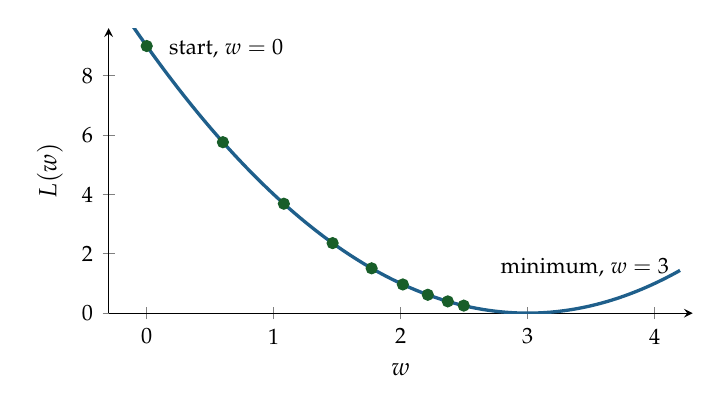
\begin{tikzpicture}
\begin{axis}[width=9cm, height=5.2cm, axis lines=left, xmin=-0.3, xmax=4.3,
  ymin=0, ymax=9.6, xlabel={$w$}, ylabel={$L(w)$}, samples=100,
  tick label style={font=\footnotesize}, label style={font=\small}]
  \addplot[very thick, accent, domain=-0.2:4.2] {(x-3)^2};
  \addplot[only marks, mark=*, mark size=2pt, st!70!black]
    coordinates {(0,9) (0.6,5.76) (1.08,3.6864) (1.464,2.3593) (1.7712,1.5099)
      (2.017,0.9664) (2.2136,0.6185) (2.3709,0.3958) (2.4967,0.2533)};
  \node[font=\footnotesize, anchor=west] at (axis cs:0.1,8.9) {start, $w=0$};
  \node[font=\footnotesize, anchor=south] at (axis cs:3.45,0.9) {minimum, $w=3$};
\end{axis}
\end{tikzpicture}
\end{center}

With learning rate 0.1, $w$ creeps toward 3 (the dots in the plot), and
the loss falls steadily. With 0.45 it gets there much faster. With 1.1,
the steps overshoot: $w$ jumps from one side of the valley to the other,
further each time, and the loss explodes.

We can see exactly why. One step changes $w$ to
$w - \eta\cdot 2(w - 3)$, so the distance from the minimum changes as
\[
  (w - 3) \;\leftarrow\; (1 - 2\eta)\,(w - 3).
\]
Every step multiplies the distance by $1 - 2\eta$: by $0.8$ for
$\eta = 0.1$, by $0.1$ for $\eta = 0.45$, and by $-1.2$ for $\eta = 1.1$,
which flips the sign and grows. Gradient descent converges here only if
$|1 - 2\eta| < 1$, that is, $0 < \eta < 1$. Real losses are not this
simple, but the lesson carries over: too small a learning rate is slow,
too large is unstable, and finding a good one takes some experiment.

\section{Many examples: stochastic gradient descent}

Our real loss is an average over half a million examples. Computing its
exact gradient would mean running all of them through the network for
every single step. Instead, each step uses a small random \emph{minibatch}
of 32 examples, and the average of their gradients, which is a noisy but
useful estimate of the true one. (The gradient of an average is the
average of the gradients, because derivatives of sums are sums of
derivatives.) This is \emph{stochastic gradient descent}: ``stochastic''
means ``random''. Many cheap, noisy steps get much further than a few
exact, expensive ones.

\section{The chain rule}

One question remains: how to compute $\pd{L}{w}$ for a weight deep inside
the network. The loss doesn't depend on such a weight directly, but
through a chain of steps: the weight affects a neuron, which affects the
scores, which affect the probabilities, which affect the loss. The
\emph{chain rule} says how derivatives combine along such a chain:

\begin{mathbox}[Chain rule]
If $L$ depends on $y$, and $y$ depends on $w$, then
\[
  \frac{dL}{dw} = \frac{dL}{dy}\cdot\frac{dy}{dw}.
\]
If $w$ affects $L$ through several in-between values $y_0, y_1, \dots$, the
contributions of all the paths add up:
\[
  \pd{L}{w} = \sum_i \pd{L}{y_i}\,\pd{y_i}{w} .
\]
\end{mathbox}

In words: the effect of a small change in $w$ on $L$ is the effect of $w$
on $y$, times the effect of $y$ on $L$. If changing $w$ by $0.01$ changes
$y$ by $0.03$ ($dy/dw = 3$), and changing $y$ by $0.03$ changes $L$ by
$0.06$ ($dL/dy = 2$), then changing $w$ by $0.01$ changes $L$ by $0.06$,
and $dL/dw = 6 = 2\cdot 3$.

Applying the chain rule backwards through the network, one layer at a
time, is called \emph{backpropagation}. It is the subject of the next
chapter.

% ===========================================================================
\chapter{Backpropagation}

We now work out, for one example, the partial derivative of the loss with
respect to every parameter. The plan is to go backwards through the
forward pass, from the loss to the input. At each stage we already know
the derivatives with respect to that stage's outputs, and we use the chain
rule to get the derivatives with respect to its inputs and its parameters.

\begin{center}
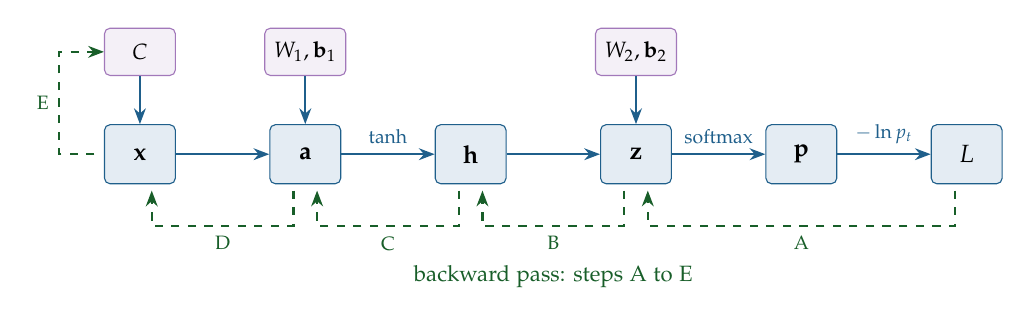
\begin{tikzpicture}[
  v/.style={draw=accent, fill=titlebg, rounded corners=2pt, minimum width=0.9cm,
    minimum height=0.75cm, font=\small},
  p/.style={draw=ty!70, fill=ty!8, rounded corners=2pt, minimum width=0.9cm,
    minimum height=0.6cm, font=\footnotesize},
  f/.style={-{Stealth[length=2mm]}, accent, thick},
  b/.style={-{Stealth[length=2mm]}, st!70!black, thick, dashed}]
  \node[v] (x) at (0,0) {$\vect{x}$};
  \node[v] (a) at (2.1,0) {$\vect{a}$};
  \node[v] (h) at (4.2,0) {$\vect{h}$};
  \node[v] (z) at (6.3,0) {$\vect{z}$};
  \node[v] (pp) at (8.4,0) {$\vect{p}$};
  \node[v] (L) at (10.5,0) {$L$};
  \node[p] (C) at (0,1.3) {$C$};
  \node[p] (W1) at (2.1,1.3) {$W_1, \vect{b}_1$};
  \node[p] (W2) at (6.3,1.3) {$W_2, \vect{b}_2$};
  \draw[f] (C) -- (x);
  \draw[f] (W1) -- (a);
  \draw[f] (W2) -- (z);
  \draw[f] (x) -- (a);
  \draw[f] (a) -- node[above, font=\scriptsize] {tanh} (h);
  \draw[f] (h) -- (z);
  \draw[f] (z) -- node[above, font=\scriptsize] {softmax} (pp);
  \draw[f] (pp) -- node[above, font=\scriptsize] {$-\ln p_t$} (L);
  \foreach \from/\to/\lab in {L/z/A, z/h/B, h/a/C, a/x/D} {
    \draw[b] ($(\from.south)+(-0.15,-0.08)$) -- ++(0,-0.45) -| node[pos=0.25, below, font=\scriptsize] {\lab} ($(\to.south)+(0.15,-0.08)$);
  }
  \draw[b] ($(x.west)+(-0.12,0)$) -- ++(-0.45,0) |- node[pos=0.25, left, font=\scriptsize] {E} (C.west);
  \node[font=\footnotesize, text=st!70!black] at (5.25,-1.55) {backward pass: steps A to E};
\end{tikzpicture}
\end{center}

A word on notation: for any value $v$ in the network we write
$\pd{L}{v}$, ``how much the loss changes per unit change of $v$''. In the
code, the same quantity is called \code{dv}: \code{dz}, \code{dh} and so
on. For a vector, it is a vector of the same length, one partial
derivative per component.

\section{The gradients container}

Each example produces a gradient for every parameter. We add the
gradients of all examples in a minibatch together, and use their average
for the update. The container has one zero-filled matrix or vector per
parameter, with the same shape:

\begin{addbefore}{next_letter_model.nex}{before the model class}{class Next_Letter_Model}
-- Zero-filled containers with the same shapes as the model's parameters.
-- During a minibatch, each example adds its gradients here.
class Gradients
create
  make(model: Next_Letter_Model) do
    c := zero_matrix(Vocabulary.SIZE, model.emb_dim)
    w1 := zero_matrix(model.hidden, model.context * model.emb_dim)
    b1 := zeros(model.hidden)
    w2 := zero_matrix(Vocabulary.SIZE, model.hidden)
    b2 := zeros(Vocabulary.SIZE)
  end
feature
  c: Array[Array[Real]]
  w1: Array[Array[Real]]
  b1: Array[Real]
  w2: Array[Array[Real]]
  b2: Array[Real]
end
\end{addbefore}

\section{Step A: softmax and cross-entropy}

The loss is $L = -\ln p_t$ with $p_t = e^{z_t}/S$, where
$S = \sum_j e^{z_j}$. The logarithm of a quotient is a difference of
logarithms, and $\ln e^{z_t} = z_t$, so
\[
  L = -\ln\frac{e^{z_t}}{S} = -z_t + \ln S .
\]
Now take the partial derivative with respect to one score $z_i$. The first
term, $-z_t$, gives $-1$ if $i = t$, and 0 otherwise. For the second, the
chain rule with $(\ln S)' = 1/S$ gives
\[
  \pd{\ln S}{z_i} = \frac{1}{S}\pd{S}{z_i} = \frac{e^{z_i}}{S} = p_i ,
\]
because only the term $e^{z_i}$ of the sum $S$ depends on $z_i$. So:

\begin{mathbox}[Step A]
\[
  \pd{L}{z_i} = p_i - y_i,
  \qquad\text{where } y_i = \begin{cases} 1 & \text{if } i = t\\ 0 & \text{otherwise.}\end{cases}
\]
\end{mathbox}

This is a beautifully simple result: the gradient is ``what the model
said'' minus ``what it should have said''. For example, if the model gives
probabilities $(0.7, 0.2, 0.1)$ and the right answer is the second symbol,
the gradient is $(0.7, -0.8, 0.1)$. Gradient descent \emph{subtracts} the
gradient, so the right answer's score goes up, and every wrong answer's
score goes down in proportion to how much probability it wrongly took. And
the gradient is small when the model is already nearly right.

In code: copy the probabilities, and subtract 1 at the target. This is the
start of the \code{backward} method; the next boxes continue it.

\begin{addbefore}{next_letter_model.nex}{before num_parameters}{  num_parameters(): Integer do}
  -- Add one example's gradients into g, by the chain rule, from the
  -- loss back to the input:
  --   loss -> logits -> W2, b2, h -> tanh -> W1, b1, x -> C
  backward(fp: Forward_Pass, target: Integer, g: Gradients)
  require
    valid_target: target >= 0 and target < Vocabulary.SIZE
  do
    -- Step A: softmax followed by cross-entropy has a very simple
    -- gradient with respect to the logits:
    --     dL/dz[i] = p[i] - (1 if i is the target, else 0)
    let dz: Array[Real] := fp.probs.clone()
    dz.set(target, dz.get(target) - 1.0)
\end{addbefore}

\section{Step B: the output layer}

The scores are $z_i = \sum_j W_{2,ij}\,h_j + b_{2,i}$. We know
$\pd{L}{z_i}$ from step A, and we want the derivatives with respect to
$W_2$, $\vect{b}_2$ and $\vect{h}$.

A weight $W_{2,ij}$ affects only one score, $z_i$, and
$\pd{z_i}{W_{2,ij}} = h_j$. A bias $b_{2,i}$ also affects only $z_i$,
with $\pd{z_i}{b_{2,i}} = 1$. But a hidden value $h_j$ affects
\emph{every} score, through the weights $W_{2,ij}$, so by the chain rule
its contributions add up over all the scores:

\begin{mathbox}[Step B, and the same for any layer $\vect{z} = W\vect{h} + \vect{b}$]
\[
  \pd{L}{W_{2,ij}} = \pd{L}{z_i}\,h_j, \qquad
  \pd{L}{b_{2,i}} = \pd{L}{z_i}, \qquad
  \pd{L}{h_j} = \sum_i \pd{L}{z_i}\,W_{2,ij} .
\]
\end{mathbox}

Look at these one row $i$ at a time. Row $i$ of the gradient of $W_2$ is
the vector $\vect{h}$ times the number $\pd{L}{z_i}$. And
$\pd{L}{\vect{h}}$ is the sum, over all rows $i$, of row $i$ of $W_2$
times $\pd{L}{z_i}$. Both are exactly what \code{add_scaled} does:

\begin{continued}{next_letter_model.nex}
    -- Step B: output layer, z = W2·h + b2.
    --     dW2[i][j] += dz[i] * h[j]     db2[i] += dz[i]
    --     dh[j]     += dz[i] * W2[i][j]
    let dh: Array[Real] := zeros(hidden)
    from
      let i: Integer := 0
    until
      i = Vocabulary.SIZE
    do
      add_scaled(g.w2.get(i), dz.get(i), fp.h)
      g.b2.set(i, g.b2.get(i) + dz.get(i))
      add_scaled(dh, dz.get(i), w2.get(i))
      i := i + 1
    end
\end{continued}

Note that we \emph{add} into \code{g}, rather than overwrite it, so that
the gradients of all the examples in a minibatch accumulate.

\section{Step C: through tanh}

Each hidden value is $h_j = \tanh(a_j)$, and depends only on its own
$a_j$. By the chain rule and the derivative of $\tanh$ from Chapter~6:

\begin{mathbox}[Step C]
\[
  \pd{L}{a_j} = \pd{L}{h_j}\,\tanh'(a_j) = \pd{L}{h_j}\,\bigl(1 - h_j^2\bigr).
\]
\end{mathbox}

We kept $\vect{h}$ from the forward pass, so this is cheap. It also shows
why the starting weights mattered: if a neuron is deep in a flat part of
$\tanh$, $h_j$ is close to $\pm 1$, the factor $1 - h_j^2$ is close to 0,
and almost no gradient gets through to the layer below. That neuron
hardly learns.

\begin{continued}{next_letter_model.nex}
    -- Step C: through tanh. tanh'(a) = 1 - tanh(a)^2 = 1 - h^2, and
    -- we already have h, so this costs almost nothing.
    let da: Array[Real] := []
    from
      let j: Integer := 0
    until
      j = hidden
    do
      let hj: Real := fp.h.get(j)
      da.add(dh.get(j) * (1.0 - hj * hj))
      j := j + 1
    end
\end{continued}

\section{Step D: the hidden layer}

The hidden layer is $\vect{a} = W_1\vect{x} + \vect{b}_1$: the same kind
of layer as in step B, so the same three formulas apply, with $W_1$,
$\vect{b}_1$, $\vect{x}$ and $\pd{L}{\vect{a}}$ in place of $W_2$,
$\vect{b}_2$, $\vect{h}$ and $\pd{L}{\vect{z}}$:
\[
  \pd{L}{W_{1,ij}} = \pd{L}{a_i}\,x_j, \qquad
  \pd{L}{b_{1,i}} = \pd{L}{a_i}, \qquad
  \pd{L}{x_j} = \sum_i \pd{L}{a_i}\,W_{1,ij} .
\]

\begin{continued}{next_letter_model.nex}
    -- Step D: hidden layer, a = W1·x + b1. Same pattern as step B.
    let dx: Array[Real] := zeros(fp.x.length)
    from
      let i: Integer := 0
    until
      i = hidden
    do
      add_scaled(g.w1.get(i), da.get(i), fp.x)
      g.b1.set(i, g.b1.get(i) + da.get(i))
      add_scaled(dx, da.get(i), w1.get(i))
      i := i + 1
    end
\end{continued}

\section{Step E: the embeddings}

The input $\vect{x}$ was the embeddings of the 4 context symbols, joined:
components $0$--$7$ are the row $C_{s_1}$, components $8$--$15$ are
$C_{s_2}$, and so on. In general, component $k\cdot 8 + m$ of $\vect{x}$
is component $m$ of the row $C_{s_k}$ (counting $k$ from 0). So the
gradient of $\vect{x}$ is cut back into 4 pieces of 8, and each piece is
added to the gradient of the row it came from:

\begin{mathbox}[Step E]
\[
  \pd{L}{C_{s,m}} = \sum_{k \,:\, s_k = s} \pd{L}{x_{8k + m}}
\]
\end{mathbox}

The sum is over every position $k$ where the symbol $s$ appears in the
context. In \code{.app}, the letter \code{p} appears twice, so its row of
$C$ gets the gradients of both positions. Rows of symbols that are not in
the context get nothing from this example.

\begin{continued}{next_letter_model.nex}
    -- Step E: embeddings. x was the context letters' rows of C joined
    -- together, so cut dx back into pieces and add each piece to the
    -- row it came from. A letter that appears twice ("pp") gets both.
    from
      let k: Integer := 0
    until
      k = context
    do
      let row: Array[Real] := g.c.get(fp.ids.get(k))
      from
        let d: Integer := 0
      until
        d = emb_dim
      do
        row.set(d, row.get(d) + dx.get(k * emb_dim + d))
        d := d + 1
      end
      k := k + 1
    end
  end
\end{continued}

The final \code{end} closes the method. That is the whole of
backpropagation for our network: about fifty lines. Here are all the
steps together, written with vectors:

\begin{mathbox}[The backward pass, in summary]
\begin{align*}
  \text{A:}\quad & \pd{L}{\vect{z}} = \vect{p} - \vect{y}\\
  \text{B:}\quad & \pd{L}{W_2} = \pd{L}{\vect{z}}\,\vect{h}^{\mathsf T},\quad
                   \pd{L}{\vect{b}_2} = \pd{L}{\vect{z}},\quad
                   \pd{L}{\vect{h}} = W_2^{\mathsf T}\pd{L}{\vect{z}}\\
  \text{C:}\quad & \pd{L}{\vect{a}} = \pd{L}{\vect{h}} \odot (1 - \vect{h}\odot\vect{h})\\
  \text{D:}\quad & \pd{L}{W_1} = \pd{L}{\vect{a}}\,\vect{x}^{\mathsf T},\quad
                   \pd{L}{\vect{b}_1} = \pd{L}{\vect{a}},\quad
                   \pd{L}{\vect{x}} = W_1^{\mathsf T}\pd{L}{\vect{a}}\\
  \text{E:}\quad & \pd{L}{C_{s}} \mathrel{+}= \text{the pieces of } \pd{L}{\vect{x}} \text{ at the positions of } s
\end{align*}
Here $\odot$ multiplies vectors component by component, and
$\vect{u}\vect{v}^{\mathsf T}$ is the matrix with entries $u_i v_j$.
\end{mathbox}

But is it right? A mistake in a formula or an index here would not crash
anything. The network would simply learn badly, or not at all, and it
would be very hard to tell why. The next chapter builds a test that
catches such mistakes.

% ===========================================================================
\chapter{Checking the gradients}

We derived the gradients with the chain rule. We can also
\emph{measure} them, directly from the definition of the derivative:
nudge one parameter up a tiny bit, run the network, nudge it down, run it
again, and see how much the loss changed. If the measured and the derived
gradients agree, the backward pass is right.

\section{The math: central differences}

The most accurate simple way to measure a derivative is the
\emph{central difference}:

\begin{mathbox}[Central difference]
\[
  f'(w) \approx \frac{f(w + \varepsilon) - f(w - \varepsilon)}{2\varepsilon}
\]
with an error proportional to $\varepsilon^2$.
\end{mathbox}

Why $\varepsilon^2$? Taylor's theorem says that near $w$,
\[
  f(w \pm \varepsilon) = f(w) \pm \varepsilon f'(w) + \tfrac12\varepsilon^2 f''(w) \pm \tfrac16\varepsilon^3 f'''(w) + \dots
\]
Subtracting the two versions, the $f(w)$ and $\varepsilon^2$ terms cancel:
\[
  f(w+\varepsilon) - f(w-\varepsilon) = 2\varepsilon f'(w) + \tfrac13\varepsilon^3 f'''(w) + \dots
\]
and dividing by $2\varepsilon$ leaves $f'(w)$ plus an error of order
$\varepsilon^2$. With $\varepsilon = 10^{-5}$, that error is around
$10^{-10}$, far smaller than any mistake we are looking for. (A one-sided
difference, $(f(w+\varepsilon) - f(w))/\varepsilon$, would only be
accurate to order $\varepsilon$.)

Measuring every gradient this way would need two forward passes per
parameter, 8166 for one example, which is why we don't train like this.
But it is perfect for spot-checking a few parameters of each kind.

\section{A file of checks}

We put the gradient check, and checks for everything else we have built,
in one file that we can run at any time. First, a small class that counts
passes and failures:

\begin{newfile}{checks.nex}
-- checks.nex: executable checks for every piece of the project.
-- Run: nex checks.nex
--
-- The most important one is the gradient check. It compares the gradients
-- that backward computes with the chain rule against gradients measured
-- directly, by nudging one parameter a tiny bit and watching the loss.
-- If backpropagation has a bug, the two disagree.

intern Vector_Math
intern Vocabulary
intern Rng
intern Next_Letter_Model
intern Training_Data
intern Helpers
intern io/Path

class Checker
create
  make() do
  end
feature
  passed: Integer
  failed: Integer

  check(label: String, ok: Boolean) do
    if ok then
      passed := passed + 1
      console.print_line("PASS " + label)
    else
      failed := failed + 1
      console.print_line("FAIL " + label)
    end
  end

  close_to(label: String, expected, actual, tolerance: Real) do
    check(label + " (expected " + expected.to_string
      + ", got " + actual.to_string + ")",
      (expected - actual).abs <= tolerance)
  end

  summary() do
    console.print_line("---")
    console.print_line(passed.to_string + " passed, " + failed.to_string + " failed")
    if failed > 0 then
      exit(1)
    end
  end
end

let c: Checker := create Checker.make()

c.summary()
\end{newfile}

Every check we add goes between \code{let c} and \code{c.summary()}.
\code{summary} exits with status 1 if anything failed, so the checks can
also be run automatically.

Let's start by locking in what we built in the earlier chapters. These
checks repeat a few of the try-it results, so that if a later change
breaks something, we find out at once:

\begin{addbefore}{checks.nex}{before the summary}{c.summary()}
-- Vector math
c.close_to("dot", 32.0, dot([1.0, 2.0, 3.0], [4.0, 5.0, 6.0]), 0.0)
let a: Array[Real] := affine([[1.0, 0.0], [1.0, 1.0]], [2.0, 3.0], [0.5, -1.0])
c.check("affine", a.get(0) = 2.5 and a.get(1) = 4.0)
let s: Array[Real] := softmax([1.0, 2.0, 3.0])
c.close_to("softmax sums to 1", 1.0, sum(s), 1.0e-12)
c.close_to("softmax[2]", 0.6652409557748219, s.get(2), 1.0e-12)
c.close_to("softmax of huge scores", 0.5, softmax([1000.0, 1000.0]).get(0), 1.0e-12)
c.close_to("tanh(0.5)", 0.46211715726000974, tanh(0.5), 1.0e-12)
c.close_to("tanh(100)", 1.0, tanh(100.0), 0.0)
c.close_to("tanh(-100)", -1.0, tanh(-100.0), 0.0)
c.check("argmax", argmax([0.1, 0.7, 0.2]) = 1)
c.check("vector_text", vector_text([0.5, -0.0499, 1.0 / 3.0], 2) = "[0.50, -0.05, 0.33]")
c.check("percent", percent(0.257) = "26%")
\end{addbefore}

\begin{addbefore}{checks.nex}{before the summary}{c.summary()}
-- Random numbers
let rng: Rng := create Rng.make(42)
let mean: Real := 0.0
let square: Real := 0.0
repeat 20000 do
  let z: Real := rng.gauss()
  mean := mean + z / 20000.0
  square := square + z * z / 20000.0
end
c.close_to("gauss mean", 0.0, mean, 0.03)
c.close_to("gauss variance", 1.0, square - mean * mean, 0.05)
let r1: Rng := create Rng.make(7)
let r2: Rng := create Rng.make(7)
c.check("same seed, same numbers", r1.uniform() = r2.uniform())

-- Vocabulary
c.check("symbol_id", symbol_id(".") = 0 and symbol_id("a") = 1 and symbol_id("z") = 26)
c.check("symbol_at", symbol_at(16) = "p")
c.check("is_lowercase_word", is_lowercase_word("apple") and not is_lowercase_word("Apple")
  and not is_lowercase_word("it's"))
\end{addbefore}

\begin{addbefore}{checks.nex}{before the summary}{c.summary()}
-- Training examples
let examples: Array[Example] := make_examples(["apple"], 4)
c.check("apple gives 6 examples", examples.length = 6)
c.check("first example", examples.get(0).ids = [0, 0, 0, 0]
  and examples.get(0).target = 1)
c.check("last example ends the word", examples.get(5).ids = [16, 16, 12, 5]
  and examples.get(5).target = 0)

-- The model
let model: Next_Letter_Model := create Next_Letter_Model.make(4, 8, 64, 42)
c.check("4083 parameters", model.num_parameters = 4083)
c.check("context_ids", model.context_ids("app") = [0, 1, 16, 16])
c.check("context_ids keeps the last letters",
  model.context_ids("banana") = [14, 1, 14, 1])
c.close_to("untrained loss is near ln 27", 27.0.log, evaluate(model, examples).loss, 0.1)
\end{addbefore}

\section{The gradient check}

Now the gradient check itself. \code{loss_on} runs the model on one
example and returns its loss. \code{gradient_matches} takes one parameter,
given as a row of a parameter matrix and a column in it, nudges it by
$\pm\varepsilon$, measures the central difference, puts the parameter back
the way it was, and compares the measurement with the gradient that
\code{backward} computed.

How close must they be? The measured value has small rounding errors of
its own, so we allow a difference of $10^{-6}$, plus $10^{-4}$ of the
gradient's size for large gradients. A mistake in the backward pass, such
as a missing factor or a wrong index, typically gives a difference of 10\%
or more.

\begin{addbefore}{checks.nex}{before the line let c}{let c: Checker := create Checker.make()}
-- The loss of a model on one example.
function loss_on(model: Next_Letter_Model, ex: Example): Real do
  result := cross_entropy(model.forward(ex.ids).probs, ex.target)
end

-- Compare backward's gradient for parameter row[col] with a measured one:
--     dL/dp  is about  (L(p + eps) - L(p - eps)) / (2 eps)
function gradient_matches(model: Next_Letter_Model, ex: Example, row: Array[Real],
  col: Integer, analytic: Real): Boolean do
  let eps: Real := 1.0e-5
  let saved: Real := row.get(col)
  row.set(col, saved + eps)
  let up: Real := loss_on(model, ex)
  row.set(col, saved - eps)
  let down: Real := loss_on(model, ex)
  row.set(col, saved)
  let numeric: Real := (up - down) / (2.0 * eps)
  result := (numeric - analytic).abs <= 1.0e-6 + 1.0e-4 * numeric.abs
end
\end{addbefore}

The vectors $\vect{b}_1$ and $\vect{b}_2$ are passed as the ``row''
themselves. For each parameter, we test a couple of entries. For $C$ we
test the row of \code{p}, which appears twice in the context \code{.app},
to check that both of its gradients are added up.

\begin{addbefore}{checks.nex}{before the summary}{c.summary()}
-- The gradient check, on one example, for a few parameters of every kind.
let ex: Example := examples.get(3)            -- ".app" -> "l"
let grads: Gradients := create Gradients.make(model)
model.backward(model.forward(ex.ids), ex.target, grads)
c.check("gradient of b2",
  gradient_matches(model, ex, model.b2, 12, grads.b2.get(12))
    and gradient_matches(model, ex, model.b2, 5, grads.b2.get(5)))
c.check("gradient of W2",
  gradient_matches(model, ex, model.w2.get(12), 3, grads.w2.get(12).get(3))
    and gradient_matches(model, ex, model.w2.get(0), 40, grads.w2.get(0).get(40)))
c.check("gradient of b1",
  gradient_matches(model, ex, model.b1, 7, grads.b1.get(7)))
c.check("gradient of W1",
  gradient_matches(model, ex, model.w1.get(7), 30, grads.w1.get(7).get(30))
    and gradient_matches(model, ex, model.w1.get(63), 0, grads.w1.get(63).get(0)))
-- "p" (id 16) appears twice in ".app", so its embedding gets two gradients.
c.check("gradient of C",
  gradient_matches(model, ex, model.c.get(16), 2, grads.c.get(16).get(2))
    and gradient_matches(model, ex, model.c.get(1), 5, grads.c.get(1).get(5)))
\end{addbefore}

\runoutput{checks.nex}{checks_gradients}

All the gradients match. To convince yourself that the check really
catches mistakes, break the backward pass on purpose. For example, in
step C, change \code{(1.0 - hj * hj)} to \code{(1.0 - hj)}, and run the
checks again: the gradients of $W_1$, $\vect{b}_1$ and $C$ now fail,
while those of $W_2$ and $\vect{b}_2$, which are computed before step C,
still pass. Put it back before you go on.

% ===========================================================================
\chapter{Taking a step}

With the gradients in hand, the update is the easy part. For every
parameter $w$, gradient descent does $w \leftarrow w - \eta\,g_w$, where
$g_w$ is the average gradient over the minibatch. The container holds the
\emph{sum} of the gradients of the batch, so the average is that sum
divided by the batch size $B$:
\[
  w \;\leftarrow\; w - \frac{\eta}{B}\,\Bigl(\sum_{\text{examples}} \pd{L}{w}\Bigr).
\]
That is \code{add_scaled} once more, with the factor $s = -\eta/B$. A
matrix is updated one row at a time:

\begin{append}{next_letter_model.nex}
-- m := m + s * g, row by row.
function update_matrix(m: Array[Array[Real]], s: Real, g: Array[Array[Real]])
require
  same_rows: m.length = g.length
do
  from
    let r: Integer := 0
  until
    r = m.length
  do
    add_scaled(m.get(r), s, g.get(r))
    r := r + 1
  end
end
\end{append}

\begin{addbefore}{next_letter_model.nex}{before num_parameters}{  num_parameters(): Integer do}
  -- Gradient descent: p := p - lr * (average gradient), for every
  -- parameter. g holds sums over the batch, so divide by its size.
  step(g: Gradients, lr: Real, batch_size: Integer)
  require
    positive_rate: lr > 0.0
    positive_batch: batch_size > 0
  do
    let s: Real := -lr / batch_size.to_real
    update_matrix(c, s, g.c)
    update_matrix(w1, s, g.w1)
    add_scaled(b1, s, g.b1)
    update_matrix(w2, s, g.w2)
    add_scaled(b2, s, g.b2)
  end
\end{addbefore}

\section{The first learning}

We have every piece of training now: forward, loss, backward, step.
Before we train on a whole dictionary, let's teach the model three words,
and watch the loss fall. Each step uses all 18 examples of the three
words as its batch.

\begin{tryit}{try_learning.nex}
intern Next_Letter_Model
intern Training_Data
intern Helpers

let model: Next_Letter_Model := create Next_Letter_Model.make(4, 8, 64, 42)
let examples: Array[Example] := make_examples(["apple", "apply", "maple"], 4)
from
  let step: Integer := 0
until
  step > 300
do
  if step % 50 = 0 then
    console.print_line("step " + step.to_string.pad_start(" ", 3) + ": loss "
      + evaluate(model, examples).loss.format(4))
  end
  let g: Gradients := create Gradients.make(model)
  across examples as ex do
    model.backward(model.forward(ex.ids), ex.target, g)
  end
  model.step(g, 0.5, examples.length)
  step := step + 1
end
let probs: Array[Real] := model.forward(model.context_ids("appl")).probs
console.print_line("after \"appl\": e " + percent(probs.get(symbol_id("e")))
  + ", y " + percent(probs.get(symbol_id("y"))))
\end{tryit}
\tryoutput{try_learning}

It learns. The loss falls from about 3.3, knowing nothing, to a fraction
of that. After \code{appl}, the model has learned that \code{e} (from
\code{apple}) and \code{y} (from \code{apply}) are the two possibilities,
about equally likely, which is exactly right for these three words. The
loss cannot go to 0: with \code{appl} as the context, no model can know
for certain which of the two words is meant.

Let's add this as a check:

\begin{addbefore}{checks.nex}{before the summary}{c.summary()}
-- Training lowers the loss: learn three words by heart.
let tiny: Array[Example] := make_examples(["apple", "apply", "maple"], 4)
let before: Real := evaluate(model, tiny).loss
repeat 300 do
  let g: Gradients := create Gradients.make(model)
  across tiny as t do
    model.backward(model.forward(t.ids), t.target, g)
  end
  model.step(g, 0.5, tiny.length)
end
let after: Real := evaluate(model, tiny).loss
c.check("training lowers the loss (" + before.format(3) + " -> " + after.format(3) + ")",
  after < before / 4.0)
\end{addbefore}

% ===========================================================================
\chapter{Saving and loading}

Training on a dictionary takes a few minutes, and we don't want to do it
every time we use the model. So we save the trained model to a file, and
load it again in the program we play with.

We use JSON, a common text format for data, through Nex's
\code{data/Json} library. A model becomes a JSON object with its three
sizes and five parameter arrays:

\begin{textout}
{"context":4,"emb_dim":8,"hidden":64,"C":[[-0.38,...],...],"W1":[...],...}
\end{textout}

\code{stringify} turns a Nex \code{Map} into JSON text. Its values can be
anything, so the map's type is \code{Map[String, Any]}. Writing the file
is \code{write_text} on a \code{Path}.

\begin{addbefore}{next_letter_model.nex}{before the invariant}{invariant}
  -- Write the model as JSON. The field names match the Python version
  -- of this project, so a model trained by one can be used by the other.
  save(path: String) do
    let data: Map[String, Any] := {
      "context": context, "emb_dim": emb_dim, "hidden": hidden,
      "C": c, "W1": w1, "b1": b1, "W2": w2, "b2": b2
    }
    let json: Json := create Json.make()
    create Path.make(path).write_text(json.stringify(data))
  end
\end{addbefore}

Loading is the reverse, with one complication. \code{parse} can return
any kind of JSON value, so its result has type \code{Any}, and so does
everything inside it. To use a value as a number or an array, we must
narrow it to that type with \code{convert}, which checks the actual type
at run time:
\code{if convert value to n: Integer then ... end} runs the \code{then}
branch, with \code{n} as an \code{Integer}, only if the value really is
one. Four small functions do this for each shape of value we expect, and
raise an error for anything else:

\begin{append}{next_letter_model.nex}
-- Reading numbers back out of parsed JSON, where every value is an Any.

function json_integer(value: Any): Integer do
  if convert value to n: Integer then
    result := n
  else
    raise "expected an integer in the model file"
  end
end

function json_real(value: Any): Real do
  if convert value to r: Real then
    result := r
  elseif convert value to n: Integer then
    result := n.to_real   -- a JSON number written without a decimal point
  else
    raise "expected a number in the model file"
  end
end

function json_vector(value: Any): Array[Real] do
  if convert value to items: Array[Any] then
    across items as item do
      result.add(json_real(item))
    end
  else
    raise "expected a list of numbers in the model file"
  end
end

function json_matrix(value: Any): Array[Array[Real]] do
  if convert value to rows: Array[Any] then
    across rows as row do
      result.add(json_vector(row))
    end
  else
    raise "expected a list of rows in the model file"
  end
end
\end{append}

Loading a model is a second way of creating one, so it is a second
constructor, next to \code{make}: \code{create Next_Letter_Model.from_file("model.json")}.
The class invariant is checked when it finishes, so a file with the
wrong shapes is rejected right away.

\begin{addbefore}{next_letter_model.nex}{as a second constructor, after make}{feature|  context: Integer   -- how many previous letters the model sees}
  -- A trained model, read back from a file written by save.
  from_file(path: String) do
    let json: Json := create Json.make()
    let text: String := create Path.make(path).read_text()
    if convert json.parse(text) to data: Map[String, Any] then
      context := json_integer(data.get("context"))
      emb_dim := json_integer(data.get("emb_dim"))
      hidden := json_integer(data.get("hidden"))
      c := json_matrix(data.get("C"))
      w1 := json_matrix(data.get("W1"))
      b1 := json_vector(data.get("b1"))
      w2 := json_matrix(data.get("W2"))
      b2 := json_vector(data.get("b2"))
    else
      raise "not a model file: " + path
    end
  end
\end{addbefore}

One last detail before we can test this. The \code{nex} command starts
programs from its own installation folder, so a file name like
\code{model.json} would be looked for there, not in our project folder.
\code{nex} records the folder it was started from, and every program can
ask for it: \code{program}, which, like \code{console}, every Nex program
has without creating it, describes the running program, and
\code{program.working_directory} is that folder. We use it to turn a
relative file name into a full one:

\begin{append}{helpers.nex}
-- The full path of a file the user named. The `nex` launcher runs
-- programs from its own installation folder, so a relative name is
-- resolved against the folder the program was started from.
function user_path(raw: String): String do
  if raw.starts_with("/") then
    result := raw
  else
    result := program.working_directory + "/" + raw
  end
end
\end{append}

The check saves the model we trained in the previous chapter, loads it
back, compares the parameters, and deletes the file:

\begin{addbefore}{checks.nex}{before the summary}{c.summary()}
-- Saving and loading give back the same model.
let file: String := user_path("checks_model.json")
model.save(file)
let loaded: Next_Letter_Model := create Next_Letter_Model.from_file(file)
c.check("save and load", loaded.w1 = model.w1 and loaded.c = model.c
  and loaded.b2 = model.b2)
create Path.make(file).delete()
\end{addbefore}

\runoutput{checks.nex}{checks_save}

% ===========================================================================
\chapter{The training program}

Time to put everything together into a program that trains a model on a
whole word list.

\section{Training and validation}

There is a trap in measuring a model on the same examples it learned
from: a model with enough parameters could memorize them, and score well
without having learned anything general. That is called
\emph{overfitting}. So we hold back 10\% of the words, never train on
them, and measure the model on those, the \emph{validation} set. If the
training loss keeps falling while the validation loss starts rising, the
model is memorizing.

We split \emph{words}, not examples. If we split examples, the model
could train on \code{.app}\,$\to$\,\code{l} and be tested on
\code{appl}\,$\to$\,\code{e} from the same word, which is a little like
seeing the exam questions in advance.

\section{The settings}

The program's settings, with their defaults, are read from the command
line: \code{nex train.nex --steps 5000 --hidden 128}, say. Start the file
with the interns, and a class that holds the settings:

\begin{newfile}{train.nex}
-- train.nex: train the next-letter model on a list of words.
--
--   nex train.nex                         -- uses /usr/share/dict/words
--   nex train.nex --words mywords.txt     -- any file with one word per line
--   nex train.nex --steps 5000            -- quicker, rougher model
--
-- It saves the trained model to model.json (change this with --out). The
-- model is also saved at every progress report, so stopping early with
-- Ctrl-C keeps the model as of the last report.
--
-- Each training step is the classic loop:
--   forward pass -> loss -> backpropagation -> parameter update
-- on a small random minibatch (stochastic gradient descent).

intern Vector_Math
intern Vocabulary
intern Rng
intern Next_Letter_Model
intern Training_Data
intern Helpers
intern io/Path
intern time/Date_Time

-- The settings of one training run, read from the command line.
class Options
create
  from_command_line(args: Array[String]) do
    words := "/usr/share/dict/words"
    out := "model.json"
    steps := 20000
    batch := 32
    lr := 0.3
    context := 4
    emb := 8
    hidden := 64
    seed := 42
\end{newfile}

The constructor continues by going through the arguments in pairs, an
option name and its value. \code{case}\,\dots\,\code{of} picks the branch
whose string matches.

\begin{continued}{train.nex}
    from
      let i: Integer := 0
    until
      i >= args.length
    do
      if i + 1 >= args.length then
        raise "missing value after " + args.get(i)
      end
      let value: String := args.get(i + 1)
      case args.get(i) of
        "--words"   then words := value
        "--out"     then out := value
        "--steps"   then steps := value.to_integer
        "--batch"   then batch := value.to_integer
        "--lr"      then lr := value.to_real
        "--context" then context := value.to_integer
        "--emb"     then emb := value.to_integer
        "--hidden"  then hidden := value.to_integer
        "--seed"    then seed := value.to_integer
        else raise "unknown option " + args.get(i)
      end
      i := i + 2
    end
  end
feature
  words: String    -- word list, one word per line
  out: String      -- where to save the trained model
  steps: Integer   -- number of minibatch updates
  batch: Integer   -- minibatch size
  lr: Real         -- learning rate (a tenth of it for the last 25%)
  context: Integer -- how many previous letters the model sees
  emb: Integer     -- embedding size
  hidden: Integer  -- hidden neurons
  seed: Integer    -- random seed, so runs can be repeated
invariant
  positive_sizes: steps > 0 and batch > 0 and context > 0 and emb > 0 and hidden > 0
  positive_rate: lr > 0.0
end
\end{continued}

The invariant rejects nonsense settings, such as \code{--steps 0} or a
negative learning rate, before any work is done. We'll also want to show
how long training has taken:

\begin{append}{train.nex}
-- Seconds since `start`, a time in milliseconds.
function seconds_since(start: Integer): Real do
  result := (create Date_Time.now().epoch_millis() - start).to_real / 1000.0
end
\end{append}

\section{Preparing the data}

The main function starts by reading the settings and the word list, and
splitting the words. \code{take(n)} gives the first $n$ elements of an
array, and \code{drop(n)} all the others.

\begin{append}{train.nex}
function main() do
  let opts: Options := create Options.from_command_line(program.arguments)
  let rng: Rng := create Rng.make(opts.seed)

  let words_path: Path := create Path.make(user_path(opts.words))
  if not words_path.exists() then
    console.print_line("Word list not found: " + opts.words)
    console.print_line("Pass one with --words (one word per line).")
    exit(1)
  end
  let words: Array[String] := load_words(words_path.path)
  if words.length < 10 then
    console.print_line("Too few usable lowercase words in " + opts.words)
    exit(1)
  end

  -- Hold back 10% of the WORDS for validation. Then we measure how well
  -- the model does on words it has never seen.
  shuffle(rng, words)
  let n_val: Integer := words.length / 10
  let val_words: Array[String] := words.take(n_val)
  let train_words: Array[String] := words.drop(n_val)
\end{append}

Then it makes the examples and the model, and reports the starting loss.
Evaluating on all the validation examples after every thousand steps
would slow training down, so we evaluate on a random sample of 3000,
which is close enough.

\begin{continued}{train.nex}
  let train: Array[Example] := make_examples(train_words, opts.context)
  let val: Array[Example] := make_examples(val_words, opts.context)
  -- Evaluating on 3000 random validation examples is quick and close enough.
  shuffle(rng, val)
  let val_sample: Array[Example] := val.take(3000)

  let model: Next_Letter_Model :=
    create Next_Letter_Model.make(opts.context, opts.emb, opts.hidden, opts.seed)
  console.print_line(train_words.length.to_string + " training words -> "
    + train.length.to_string + " examples; "
    + val_words.length.to_string + " validation words")
  console.print_line("model has " + model.num_parameters.to_string + " parameters (context="
    + opts.context.to_string + ", emb=" + opts.emb.to_string
    + ", hidden=" + opts.hidden.to_string + ")")

  let before: Evaluation := evaluate(model, val_sample)
  console.print_line("before training: val loss " + before.loss.format(3)
    + " (guessing uniformly would give " + Vocabulary.SIZE.to_real.log.format(3) + ")")
  console.print_line("")
\end{continued}

\section{The training loop}

Each step builds a minibatch of randomly chosen training examples, runs
forward and backward on each, and updates the model once with their
summed gradients. These few lines are the heart of the whole project.

We use one more trick, a \emph{learning-rate schedule}: the full learning
rate for the first 75\% of the steps, then a tenth of it. Big steps make
fast progress early on, but near the bottom of the valley they bounce from
side to side, like the $\eta = 1.1$ example of Chapter~12 but milder.
Smaller steps let the model settle.

The rate for each step is chosen with \code{when ... then ... else ...
end}, an \code{if} that gives a value.

\begin{continued}{train.nex}
  let report_every: Integer := (opts.steps / 20).max(1)
  let running_loss: Real := 0.0
  let start: Integer := create Date_Time.now().epoch_millis()

  from
    let step: Integer := 1
  until
    step > opts.steps
  do
    -- Learning-rate schedule: big steps first for fast progress, then
    -- smaller steps to settle into the bottom of the valley.
    let lr: Real := when step * 4 <= opts.steps * 3 then opts.lr else opts.lr / 10.0 end

    -- One minibatch of randomly chosen examples: the "stochastic" in
    -- stochastic gradient descent.
    let grads: Gradients := create Gradients.make(model)
    repeat opts.batch do
      let ex: Example := train.get(rng.below(train.length))
      let fp: Forward_Pass := model.forward(ex.ids)                     -- forward
      running_loss := running_loss + cross_entropy(fp.probs, ex.target) -- loss
      model.backward(fp, ex.target, grads)                              -- backprop
    end
    model.step(grads, lr, opts.batch)                                   -- update
\end{continued}

Twenty times during training, the loop prints a progress report: the
average loss on the training examples since the last report, the loss and
accuracy on the validation sample, and the time so far. It also saves the
model, so that stopping early with Ctrl-C loses at most one report's
worth of training.

\begin{continued}{train.nex}
    if step % report_every = 0 or step = opts.steps then
      let train_loss: Real := running_loss / (report_every * opts.batch).to_real
      running_loss := 0.0
      let val_now: Evaluation := evaluate(model, val_sample)
      console.print_line("step " + step.to_string.pad_start(" ", 6) + "/" + opts.steps.to_string
        + "  lr " + lr.format(3)
        + "  train loss " + train_loss.format(3)
        + "  val loss " + val_now.loss.format(3)
        + "  val accuracy " + (val_now.accuracy * 100.0).format(1).pad_start(" ", 4) + "%"
        + "  [" + seconds_since(start).format(0).pad_start(" ", 5) + "s]")
      model.save(user_path(opts.out))
    end
    step := step + 1
  end

  console.print_line("")
  console.print_line("saved to " + opts.out + ". Try:  nex play.nex")
end
\end{continued}

And finally, the line that runs it all:

\begin{append}{train.nex}
main()
\end{append}

\section{Running it}

A quick run first, with a tenth of the default steps, to check that
everything works:

\runoutput{train.nex --steps 2000 --out quick.json}{train_quick}

Now the real thing. With the defaults, 20000 steps of 32 examples, the
model sees 640,000 examples, a little more than the whole training set
once. It takes a few minutes:

\begin{shell}
nex train.nex
\end{shell}

\begin{textout}
57465 training words -> 533799 examples; 6384 validation words
model has 4083 parameters (context=4, emb=8, hidden=64)
before training: val loss 3.297 (guessing uniformly would give 3.296)

step   1000/20000  lr 0.300  train loss 2.526  val loss 2.392  val accuracy 27.5%  [   10s]
step   2000/20000  lr 0.300  train loss 2.371  val loss 2.328  val accuracy 28.8%  [   17s]
step   3000/20000  lr 0.300  train loss 2.345  val loss 2.280  val accuracy 29.0%  [   25s]
...
step  14000/20000  lr 0.300  train loss 2.233  val loss 2.218  val accuracy 29.8%  [  118s]
step  15000/20000  lr 0.300  train loss 2.255  val loss 2.212  val accuracy 31.2%  [  127s]
step  16000/20000  lr 0.030  train loss 2.153  val loss 2.132  val accuracy 32.3%  [  138s]
step  17000/20000  lr 0.030  train loss 2.134  val loss 2.128  val accuracy 32.7%  [  148s]
step  18000/20000  lr 0.030  train loss 2.126  val loss 2.121  val accuracy 32.9%  [  157s]
step  19000/20000  lr 0.030  train loss 2.143  val loss 2.123  val accuracy 32.9%  [  166s]
step  20000/20000  lr 0.030  train loss 2.130  val loss 2.118  val accuracy 33.1%  [  174s]

saved to model.json. Try:  nex play.nex
\end{textout}

\begin{center}
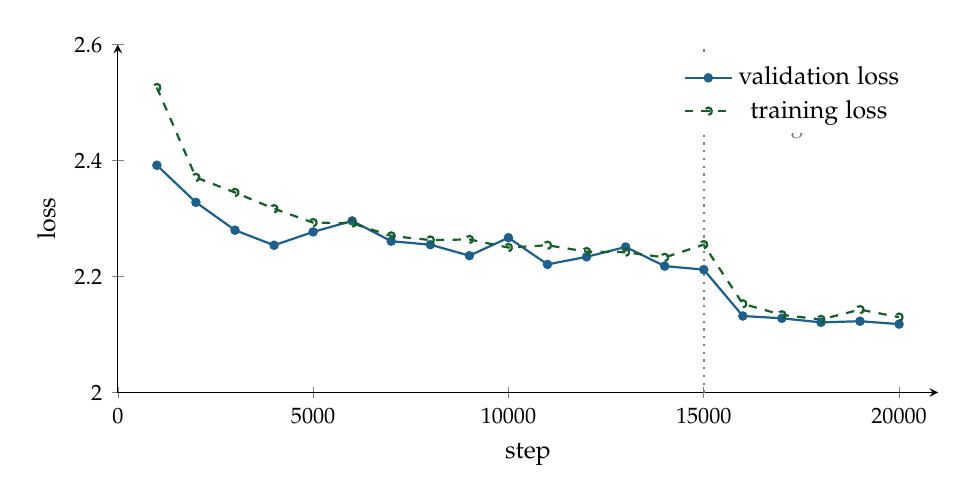
\begin{tikzpicture}
\begin{axis}[width=12cm, height=6cm, axis lines=left, xmin=0, xmax=21000,
  ymin=2.0, ymax=2.6, xlabel={step}, ylabel={loss},
  scaled x ticks=false, xtick={0,5000,10000,15000,20000},
  xticklabels={0,5000,10000,15000,20000},
  legend style={draw=none, font=\small, at={(0.97,0.97)}, anchor=north east},
  tick label style={font=\footnotesize}, label style={font=\small}]
  \addplot[thick, accent, mark=*, mark size=1.3pt] coordinates {
    (1000,2.392) (2000,2.328) (3000,2.280) (4000,2.254) (5000,2.277)
    (6000,2.296) (7000,2.261) (8000,2.255) (9000,2.236) (10000,2.267)
    (11000,2.221) (12000,2.234) (13000,2.251) (14000,2.218) (15000,2.212)
    (16000,2.132) (17000,2.128) (18000,2.121) (19000,2.123) (20000,2.118)};
  \addlegendentry{validation loss}
  \addplot[thick, st!70!black, dashed, mark=o, mark size=1.3pt] coordinates {
    (1000,2.526) (2000,2.371) (3000,2.345) (4000,2.317) (5000,2.293)
    (6000,2.292) (7000,2.270) (8000,2.263) (9000,2.264) (10000,2.250)
    (11000,2.254) (12000,2.243) (13000,2.242) (14000,2.233) (15000,2.255)
    (16000,2.153) (17000,2.134) (18000,2.126) (19000,2.143) (20000,2.130)};
  \addlegendentry{training loss}
  \draw[gray, dotted, thick] (axis cs:15000,2.0) -- (axis cs:15000,2.6);
  \node[font=\footnotesize, anchor=south west, text=cm] at (axis cs:15200,2.42) {learning rate $\div 10$};
\end{axis}
\end{tikzpicture}
\end{center}

How to read this:
\begin{itemize}
  \item \textbf{The loss falls fast, then slowly.} From 3.30 (knowing
    nothing) to 2.39 within the first thousand steps, and then only slowly
    to 2.21 by step 15000, bouncing up and down because every minibatch is
    different.
  \item \textbf{The learning-rate drop helps at once.} At step 16000, just
    after the drop, the loss falls from about 2.21 to 2.13: the smaller
    steps settle into the valley instead of bouncing around in it.
  \item \textbf{No overfitting.} The training and validation losses stay
    close together all the way. With 4083 parameters and over half a
    million examples, the model cannot memorize the words; it can only
    learn general spelling patterns. In fact a model this small is more
    likely \emph{underfitting}: too small to capture everything there is
    to learn. Try \code{--hidden 128}.
  \item \textbf{What the numbers mean.} The final loss of 2.12 is a
    perplexity of $e^{2.12}\approx 8.3$: on average, the model is about as
    unsure as if it were choosing among 8 equally likely symbols, instead
    of 27. Its top guess is right 33\% of the time, against 3.7\% for
    guessing. That might sound low, but even a perfect model would be far
    from 100\%: after \code{app}, both \code{l} (apple) and \code{r}
    (approve) are right for some words.
\end{itemize}

% ===========================================================================
\chapter{Playing with the model}

The last program loads the trained model and uses it to complete words.

\section{Predictions}

First, a method that gives every symbol with its probability, most likely
first. A small class holds one such pair:

\begin{addbefore}{next_letter_model.nex}{before the model class}{class Next_Letter_Model}
-- One row of a prediction: a symbol and its probability.
class Prediction
create
  make(symbol: String, probability: Real) do
    this.symbol := symbol
    this.probability := probability
  end
feature
  symbol: String
  probability: Real
end
\end{addbefore}

\code{sort} takes a comparison function, written here with \code{fn}: it
returns a negative number if \code{a} should come first, and a positive
one if \code{b} should. Comparing \code{b} with \code{a}, rather than
\code{a} with \code{b}, sorts from most to least likely.

\begin{addbefore}{next_letter_model.nex}{before num_parameters}{  num_parameters(): Integer do}
  -- Every symbol with its probability, most likely first.
  predict(prefix: String): Array[Prediction]
  require
    known_symbols: is_lowercase_word(prefix) or prefix = ""
  do
    let probs: Array[Real] := forward(context_ids(prefix)).probs
    let unsorted: Array[Prediction] := []
    from
      let i: Integer := 0
    until
      i = Vocabulary.SIZE
    do
      unsorted.add(create Prediction.make(symbol_at(i), probs.get(i)))
      i := i + 1
    end
    result := unsorted.sort(fn(a, b: Prediction): Integer do
      result := b.probability.compare(a.probability)
    end)
  ensure
    every_symbol: result.length = Vocabulary.SIZE
  end
\end{addbefore}

One more check, that the model trained on three words in Chapter~15 has
learned the possible continuations of \code{appl}:

\begin{addbefore}{checks.nex}{before the summary}{c.summary()}
-- Predictions come sorted, and say what was learned.
let ranked: Array[Prediction] := model.predict("appl")
c.check("predictions are sorted", ranked.get(0).probability >= ranked.get(1).probability
  and ranked.get(1).probability >= ranked.get(26).probability)
c.check("it learned: after \"appl\" comes e or y",
  ranked.get(0).symbol = "e" or ranked.get(0).symbol = "y")
\end{addbefore}

\runoutput{checks.nex}{checks_final}

That is the complete set of checks.

\section{The play program}

The program has two modes. Given some word beginnings on the command
line, it completes each one by always taking the model's top choice. With
no arguments, it lets you steer, as in the session at the start of this
tutorial. The file starts with the interns and two constants:

\begin{newfile}{play.nex}
-- play.nex: type the start of a word and let the model finish it, letter
-- by letter.
--
--   nex play.nex                    -- interactive
--   nex play.nex app hel qu         -- complete each prefix and exit
--   nex play.nex --model other.json
--
-- Interactive keys, after each suggestion:
--   Enter      accept the suggested letter
--   n          show the next most likely letter instead
--   letters    type them yourself (e.g. "r" to steer "app" toward "appr...")
--   q          give up on this word and start a new one

intern Vocabulary
intern Next_Letter_Model
intern Helpers
intern io/Path

class Play
feature
  MAX_LEN = 30        -- safety stop, in case the model never predicts "."
  ALTERNATIVES = 5    -- how many suggestions "n" cycles through
end
\end{newfile}

Completing a word by always taking the top choice is called
\emph{greedy} decoding. It stops when the top choice is the end marker,
or, as a safety net, when the word gets very long.

\begin{append}{play.nex}
function describe(symbol: String): String do
  result := when symbol = Vocabulary.END then "<end of word>" else symbol end
end

-- Always take the single most likely symbol until the model says ".".
function greedy_complete(model: Next_Letter_Model, prefix: String): String do
  result := prefix
  let done: Boolean := false
  from
  until
    done or result.length >= Play.MAX_LEN
  do
    let best: String := model.predict(result).get(0).symbol
    if best = Vocabulary.END then
      done := true
    else
      result := result + best
    end
  end
end
\end{append}

For the interactive mode, two helpers: one lists the other top choices,
and one reads a line of input. \code{read_line} returns \code{nil} at the
end of the input (when you press Ctrl-D), so its type is \code{?String},
``a string or nil''. The \emph{object test} \code{?line as text} is true
when \code{line} is not \code{nil}, and then gives us the string as
\code{text}.

\begin{append}{play.nex}
-- The other top choices, e.g. "r 21%, e 5%, end 3%".
function others(ranked: Array[Prediction], skip: String): String do
  let parts: Array[String] := []
  across ranked.take(Play.ALTERNATIVES) as p do
    if p.symbol /= skip then
      parts.add(when p.symbol = Vocabulary.END then "end" else p.symbol end
        + " " + percent(p.probability))
    end
  end
  result := ", ".join(parts)
end

-- Read a line, lowercased and trimmed; nil at end of input (Ctrl-D).
function ask(prompt: String): ?String do
  let line: ?String := console.read_line(prompt)
  if ?line as text then
    result := text.trim().to_lower()
  end
end
\end{append}

The interactive completion of one word shows a suggestion, reads your
answer, and acts on it, until the word is finished, abandoned, or the
input ends. \code{choice} says which of the ranked options is being
shown; \code{n} moves it to the next one.

\begin{append}{play.nex}
-- Suggest letters for one word until it is finished or abandoned.
-- Returns false when the input has ended.
function complete_interactively(model: Next_Letter_Model,
  start: String): Boolean do
  result := true
  let word: String := start
  let choice: Integer := 0     -- which of the ranked options to show
  let finished: Boolean := false
  let abandoned: Boolean := false
  from
  until
    finished or abandoned or not result or word.length >= Play.MAX_LEN
  do
    let ranked: Array[Prediction] := model.predict(word)
    let shown: Prediction := ranked.get(choice)
    let prompt: String := when shown.symbol = Vocabulary.END then
      "  " + word + "   -> looks complete (" + percent(shown.probability) + ")   "
    else
      "  " + word + "[" + shown.symbol + "]   (" + percent(shown.probability) + ")   "
    end
    console.print_line(prompt + "   others: " + others(ranked, shown.symbol))
\end{append}

\begin{continued}{play.nex}
    let answer: ?String := ask("  > ")
    if ?answer as ans then
      if ans = "" then                          -- accept the suggestion
        if shown.symbol = Vocabulary.END then
          finished := true
        else
          word := word + shown.symbol
          choice := 0
        end
      elseif ans = "n" then                     -- show the next option
        choice := (choice + 1) % Play.ALTERNATIVES
      elseif ans = "q" then                     -- abandon this word
        abandoned := true
      elseif is_lowercase_word(ans) then        -- the user types letters
        word := word + ans
        choice := 0
      else
        console.print_line("  Enter = accept, n = next option, letters = type your own, "
          + "q = new word")
      end
    else
      result := false                           -- end of input
    end
  end
  if abandoned or not result then
    console.print_line("")
  else
    console.print_line("  ==> " + word)
    console.print_line("")
  end
end
\end{continued}

The outer loop asks for the start of a word, and hands it to
\code{complete_interactively}, until you enter an empty line or the input
ends:

\begin{append}{play.nex}
function interactive(model: Next_Letter_Model) do
  console.print_line("Next-letter predictor. Type the start of a word "
    + "(empty line or Ctrl-D to quit).")
  console.print_line("After each suggestion: Enter = accept, n = next option, "
    + "letters = type your own, q = new word.")
  console.print_line("")
  let going: Boolean := true
  from
  until
    not going
  do
    let line: ?String := ask("start of word> ")
    if ?line as word then
      if word = "" then
        going := false
      elseif not is_lowercase_word(word) then
        console.print_line("  please use letters a-z only")
        console.print_line("")
      else
        going := complete_interactively(model, word)
      end
    else
      console.print_line("")
      going := false
    end
  end
end
\end{append}

Finally, \code{main} reads the command line (an optional
\code{--model} file, and any word beginnings), loads the model, and runs
one of the two modes.

\begin{append}{play.nex}
function main() do
  let args: Array[String] := program.arguments
  let model_file: String := "model.json"
  let prefixes: Array[String] := []
  from
    let i: Integer := 0
  until
    i >= args.length
  do
    if args.get(i) = "--model" and i + 1 < args.length then
      model_file := args.get(i + 1)
      i := i + 2
    else
      prefixes.add(args.get(i).to_lower())
      i := i + 1
    end
  end

  if not create Path.make(user_path(model_file)).exists() then
    console.print_line("No model at " + model_file + ". Train one first: nex train.nex")
    exit(1)
  end
  let model: Next_Letter_Model :=
    create Next_Letter_Model.from_file(user_path(model_file))
\end{append}

\begin{continued}{play.nex}
  if prefixes.is_empty then
    interactive(model)
  else
    across prefixes as prefix do
      if is_lowercase_word(prefix) then
        let ranked: Array[Prediction] := model.predict(prefix)
        let top: String := ""
        across ranked.take(3) as p do
          if top /= "" then
            top := top + ", "
          end
          top := top + describe(p.symbol) + " " + percent(p.probability)
        end
        console.print_line(prefix.pad_start(" ", 12) + " -> "
          + greedy_complete(model, prefix).pad_end(" ", 16) + "(next letter: " + top + ")")
      else
        console.print_line(prefix.pad_start(" ", 12) + " -> please use letters a-z only")
      end
    end
  end
end

main()
\end{continued}

\section{Trying it}

With the model trained in the previous chapter:

\runoutput{play.nex app thin walk qu}{play_oneshot}

After \code{thin}, the model is 72\% sure of \code{g}, and then sure that
\code{thing} is complete. After \code{walk}, it suggests \code{walking}.
But \code{app} became \code{apprate} and \code{qu} became \code{quint}:
always taking the top choice tends to produce plausible-looking words
that are not quite real, or are not the ones you meant. The interactive
mode, where you steer, works much better:

\begin{shell}
nex play.nex
\end{shell}

\begin{textout}
start of word> app
  app[r]   (23%)      others: e 19%, l 17%, o 15%, i 9%
  > l
  appl[e]   (45%)      others: i 19%, a 13%, y 11%, o 8%
  >
  apple[a]   (21%)      others: s 18%, r 11%, end 7%, n 7%
  > n
  apple[s]   (18%)      others: a 21%, r 11%, end 7%, n 7%
  >
  apples   -> looks complete (42%)      others: s 19%, t 15%, e 4%, h 4%
  >
  ==> apples
\end{textout}

Why does the model prefer \code{r} after \code{app}, when \code{apple} is
surely the most common word starting that way? Because it learned from a
dictionary, which lists every word once. ``Apple'' and ``appraise'' count
the same, and the dictionary has many more words starting with
\code{appr} (approach, approve, appropriate, \dots) and \code{appe}
(appear, append, appetite, \dots) than with \code{appl}. The model has
learned the dictionary's spelling patterns, not how often people use each
word. Trained on ordinary text, with common words appearing many times,
it would learn different preferences.

% ===========================================================================
\chapter{Where to go next}

You have built, from nothing, every part of a neural network that learns
to spell: embeddings, layers, an activation function, softmax, the
cross-entropy loss, backpropagation, a gradient check, and stochastic
gradient descent with a learning-rate schedule.

\section{What it can't do}

\begin{itemize}
  \item \textbf{It only sees four letters.} In a long word, it has
    forgotten how the word began. Raise \code{--context} to see more, at
    the cost of more parameters and slower training.
  \item \textbf{It knows spelling, not usage}, as we saw with \code{app}.
  \item \textbf{It invents words.} It learned what English words look
    like, not a list of them, so it happily completes \code{qu} to
    something word-like that isn't in the dictionary. This is the same
    behavior that makes large language models ``hallucinate'': they
    produce what is plausible, which is not always what is true.
\end{itemize}

\section{Experiments to try}

\begin{itemize}
  \item \textbf{Bigger models.} Train with \code{--hidden 128}, or
    \code{--emb 10 --context 5}, and compare the validation loss. Does the
    gap between training and validation loss grow?
  \item \textbf{Learning rates.} Try \code{--lr 0.1} and \code{--lr 1.0}.
    Which trains faster? Does either become unstable?
  \item \textbf{ReLU.} Replace $\tanh$ with the \emph{rectified linear
    unit}, $\operatorname{relu}(v) = \max(0, v)$, which is popular in deep
    networks. Its derivative is 1 for $v > 0$ and 0 otherwise. You need to
    change \code{forward} (the activation) and step C of \code{backward}
    (the derivative); then run the gradient check. (Strictly, the
    derivative at exactly $v=0$ is undefined; any choice works in
    practice.)
  \item \textbf{Temperature.} Divide the scores by a number $T$ before
    softmax: $p_i = e^{z_i/T}/\sum_j e^{z_j/T}$. With $T < 1$, the
    differences between scores grow and the model becomes more decisive;
    with $T > 1$, the probabilities even out and it becomes more
    adventurous. Then, instead of always taking the top choice, pick a
    symbol at random according to its probability (\emph{sampling}), and
    let the model invent new words.
  \item \textbf{A second hidden layer.} Add a layer
    $\vect{h}_2 = \tanh(W_3\vect{h} + \vect{b}_3)$ between the hidden
    layer and the output. The backward pass gains one more step B and C.
    The gradient check will tell you whether you got it right.
\end{itemize}

\section{From here to a language model}

The models behind today's chatbots are built from the same pieces. Their
\emph{vocabulary} has tens of thousands of \emph{tokens} (words and pieces
of words) instead of 27 symbols, each with an embedding of thousands of
numbers. Instead of joining a fixed window of four embeddings, they use a
mechanism called \emph{attention} that lets every position look back at
every earlier one, across thousands of tokens. They stack dozens of
layers, and have billions of parameters, trained on a large part of the
text on the internet with many computers working for months. But at the
end there is still a softmax over the vocabulary, trained with
cross-entropy to predict what comes next, with gradients computed by
backpropagation and applied by a variant of gradient descent. You have
written all of those by hand.

% ===========================================================================
\appendix
\chapter{The math on one page}

\begin{mathbox}[Forward pass, for context symbols $s_1,\dots,s_4$ and target $t$]
\begin{align*}
  \vect{x} &= (C_{s_1}, C_{s_2}, C_{s_3}, C_{s_4}) &
  \vect{a} &= W_1\vect{x} + \vect{b}_1 &
  \vect{h} &= \tanh(\vect{a}) \\
  \vect{z} &= W_2\vect{h} + \vect{b}_2 &
  p_i &= \frac{e^{z_i - m}}{\sum_j e^{z_j - m}},\ m = \max_j z_j &
  L &= -\ln p_t
\end{align*}
\end{mathbox}

\begin{mathbox}[Backward pass]
\begin{align*}
  \pd{L}{z_i} &= p_i - [i = t] \\
  \pd{L}{W_{2,ij}} &= \pd{L}{z_i}\,h_j, \quad
  \pd{L}{b_{2,i}} = \pd{L}{z_i}, \quad
  \pd{L}{h_j} = \sum_i \pd{L}{z_i}\,W_{2,ij} \\
  \pd{L}{a_j} &= \pd{L}{h_j}\,(1 - h_j^2) \\
  \pd{L}{W_{1,ij}} &= \pd{L}{a_i}\,x_j, \quad
  \pd{L}{b_{1,i}} = \pd{L}{a_i}, \quad
  \pd{L}{x_j} = \sum_i \pd{L}{a_i}\,W_{1,ij} \\
  \pd{L}{C_{s,m}} &= \sum_{k\,:\,s_k = s} \pd{L}{x_{k\cdot d + m}} \qquad (d = \text{embedding size})
\end{align*}
$[i = t]$ is 1 if $i = t$ and 0 otherwise.
\end{mathbox}

\begin{mathbox}[Training]
\begin{align*}
  w &\leftarrow w - \frac{\eta}{B}\sum_{\text{batch}}\pd{L}{w}
    && \text{minibatch gradient descent, batch size } B\\
  f'(w) &\approx \frac{f(w+\varepsilon) - f(w-\varepsilon)}{2\varepsilon}
    && \text{gradient check, error } O(\varepsilon^2)
\end{align*}
\end{mathbox}

\begin{mathbox}[Useful facts]
\begin{align*}
  \tanh(v) &= 1 - \frac{2}{e^{2v}+1}, \quad \tanh'(v) = 1 - \tanh^2(v) \\
  \operatorname{softmax}(\vect{z} + c) &= \operatorname{softmax}(\vect{z}) \\
  \operatorname{Var}\Bigl(\sum_{j=1}^{n} w_j x_j\Bigr) &= n\,\sigma_w^2\,\sigma_x^2
     \quad\text{(independent, mean 0), so use } \sigma_w = 1/\sqrt{n} \\
  \text{know-nothing loss} &= \ln 27 \approx 3.296, \quad
  \text{perplexity} = e^{L} \\
  \text{Box--Muller:}\quad z &= \sqrt{-2\ln u_1}\,\cos(2\pi u_2) \\
  \text{Park--Miller:}\quad \text{state} &\leftarrow 48271\cdot\text{state} \bmod (2^{31}-1)
\end{align*}
\end{mathbox}

\chapter{The Nex you met}

A reminder of the Nex features this project uses.

\begin{center}
\small
\begin{tabular}{@{}p{5.6cm}p{8.4cm}@{}}
\toprule
Feature & Example \\
\midrule
\code{intern} another file & \code{intern Helpers} loads everything in \code{helpers.nex}; no class of that name is needed \\
Class constants & \code{SIZE = 27}, read as \code{Vocabulary.SIZE} \\
\code{result} and its zero value & \code{result} starts at \code{0.0}, \code{""}, \code{[]}, \dots \\
Preconditions, postconditions & \code{require same_length: ...}, \code{ensure sums_to_one: ...} \\
Class invariants & \code{invariant state_in_range: ...} \\
\code{rescue} and \code{exception} & catching a contract violation in a try-it script \\
\code{when ... then ... else ... end} & an \code{if} that gives a value \\
Loops & \code{from ... until ... do ... end}, \code{repeat n do}, \code{across xs as x do} \\
Generic functions & \code{shuffle[T](rng: Rng, items: Array[T])} \\
Several constructors & \code{make} and \code{from_file} \\
Anonymous functions & \code{fn(a, b: Prediction): Integer do ... end} for \code{sort} \\
\code{convert} & narrowing an \code{Any} from JSON to \code{Integer}, \code{Real}, \code{Array[Any]} \\
Detachable types, object test & \code{?String}, \code{if ?line as text then} \\
\code{case ... of} & matching option names in \code{train.nex} \\
Built-in \code{Real} methods & \code{format} for printing, \code{round}, \code{log}, \code{sqrt} \\
Built-in \code{String} methods & \code{pad_start}, \code{pad_end}, \code{replicate}, \code{join}, \code{substring}, \code{trim} \\
Libraries & \code{data/Json}, \code{text/Regex}, \code{io/Path}, \code{time/Date_Time}, \code{console}, \code{program} \\
\bottomrule
\end{tabular}
\end{center}

\end{document}
